\cleardoublepage
\chapter{Stand der Technik und der Forschung}
\label{ch:Stand_der_Technik}

\textbf{Vorschlag:} Dieses Kapitel stellt die technischen Grundlagen vor, auf denen die Arbeit aufbaut. Zunächst wird beschrieben, was modulare Roboterzellen auszeichnet (Abschnitt~\ref{sec:Modulare Roboterzellen}). Anschließend werden gängige Technologien für die Kommunikation zwischen industriellen Komponenten betrachtet (Abschnitt~\ref{sec:Kommunikationstechnologien}) und verschiedene Verfahren zur Lokalisierung von Objekten vorgestellt (Abschnitt~\ref{sec:Lokalisierungstechnologien}).

\section{Art der Abschlussarbeit}
Je nach Art der Abschlussarbeit muss die Vorlage eigenständig angepasst werden. 
Der Typ der Arbeit wird auf der Titelseite in der \textit{Documentclass} in der Datei \textit{PLCM-Thesis.tex} angepasst.  

\section{Aufgabenstellung}
\begin{sloppypar}
\begin{itemize}
    \item Bei externen Arbeiten muss vorher ein Antrag zur Genehmigung der externen Arbeit gestellt werden. Hier muss der Titel der Arbeit schon feststehen und die Aufgabenstellung darf nach den Vorgaben des PLCM keinen Sperrvermerk enthalten.

    Weitere Informationen beim MechCenter unter \href{https://www.maschinenbau.tu-darmstadt.de/studieren/studierende/studium_bachelor/abschlussarbeiten_bachelor/index.de.jsp}{Bachelorarbeiten}  bzw. \href{https://www.maschinenbau.tu-darmstadt.de/studieren/studierende/studium_master/abschlussarbeit/index.de.jsp}{Masterarbeiten} \\
    oder auf dem Merkblatt Abschlussarbeiten der TU Darmstadt:
    \href{https://www.tu-darmstadt.de/media/dezernat_ii/referat_iig/fuer_pruefende/merkblaetter/info_externe_abschlussarbeiten.pdf}{Merkblatt}

    \item Die Aufgabenstellung wird vom Betreuer erstellt und muss vor Ausgabe an den Studenten von Herrn Prof. Schleich genehmigt werden. 

    \item Die Aufgabenstellung muss bei einer Bachelor-/Masterthesis auf eine Seite passen. Bei einer Aufgabenstellung eines Advanced Design Projects (ADP) bzw. Advanced Research Projects (ARP) dürfen es auch zwei Seiten sein. Auf der Aufgabenstellung steht auch der englische Titel der Arbeit. 

    \item Die Aufgabenstellung wird mit dem Studenten besprochen und ggf. angepasst. 

    \item Alles, was in der Aufgabenstellung steht, muss auch gemacht werden. Je allgemeiner formuliert, desto mehr Handlungsspielraum besteht während der Bearbeitungszeit und bei der Bewertung der Ausarbeitung.


    \item Nach Abgabe der Aufgabenstellung durch den Studenten im MechCenter, sollte der Student überprüfen, ob der Titel in \href{https://www.tucan.tu-darmstadt.de}{TUCaN} richtig eingetragen ist. 

\end{itemize}

Kontakt \href{https://www.maschinenbau.tu-darmstadt.de/studieren/mechcenter_studienbuero/pruefungsangelegenheiten/index.de.jsp}{MechCenter} -- Prüfungsangelegenheiten:\\ pruefungsmanagement@mechcenter.tu-darmstadt.de 

\end{sloppypar}


\section{Austausch von Dateien}
\begin{itemize}

    \item Zum Austausch von Dateien legt der Betreuer einen Ordner in der \href{https://next.hessenbox.de/shibboleth-ds/index.html?entityID=https%3A%2F%2Fnext.hessenbox.de%2Fshibboleth&return=https%3A%2F%2Fnext.hessenbox.de%2FShibboleth.sso%2FLogin%3FSAMLDS%3D1%26target%3Dss%253Amem%253Ab869f007763b2d33bdeb1bddb90fe9367a6913159761f53f4ed9cdc768118a2e}{next.Hessenbox} an. Dieser Ordner hat die einheitliche Ordnerstruktur mit den Unterordnern:
    \begin{itemize}
    \item 00\_Abgabe
    \item 01\_Orga
    \item 02\_Treffen
    \item 03\_Inhalt
    \item 04\_Ausarbeitung
    \item 05\_Kolloquium
    \end{itemize}
    
    
    Abgabe, Ausarbeitung, Literatur, Citavi, Präsentation, Organisatorisches, Analyse, Versuche, Veröffentlichung. 
    \item Dateinamen immer \textbf{ohne} Leerschritte schreiben. Bei Dateinamen dürfen Buchstaben a-z und A-Z, Ziffern 0-9, Minus/Bindestriche - und Unterstriche verwendet werden.  
    \item Sinnvolle Benennung für Dateien verwenden. 
    \item Zwischenversionen speichern
    \item Speicherkopien des Hessenboxordners erstellen. Dafür empfiehlt sich eine Backup Software, wie bspw. Veeam Agent.
\end{itemize}

\section{Organisatorisches zwischen Betreuer und Student}
\begin{itemize}
    \item geplante Urlaube/Abwesenheiten mitteilen
    \item Regeltermine vereinbaren
    \item klären, wie viele Seiten die Ausarbeitung etwa haben soll
    \item klären, wie viele Wochen vor finaler Endabgabe die fertige Version an den Betreuer geschickt werden soll
\end{itemize}

\section{Corporate Design}

\begin{sloppypar}
Infos zum Corporate Design der TU Darmstadt sind unter \url{https://www.intern.tu-darmstadt.de/arbeitsmittel/corporate_design_vorlagen/index.de.jsp} zu finden.\\
Dazu zählen Vorlagen, Schriften und Farben. 
\end{sloppypar}

\subsection{Vorlagen}

\begin{itemize}
    \item Die schriftliche Ausarbeitung kann in Word oder in LaTeX verfasst werden. 

    \item Über \href{https://sharelatex.tu-darmstadt.de/}{ShareLaTeX TU-Darmstadt}  können Vorlagen für Abschlussarbeiten angepasst und verwendet werden. Dabei muss die Farbe der Titelseite und der Balken auf jeder Seite auf das PLCM-Blau angepasst werden, siehe \ref{subsec:farbe}. 

    \item Weiter Infos zu \href{https://www.hrz.tu-darmstadt.de/services/it_services/sharelatex_hrz/index.de.jsp}{ShareLaTeX}

    \item Die LaTeX- bzw. Word-Vorlage sowie die PowerPoint-Vorlage werden über die Hessenbox zur Verfügung gestellt. 
\end{itemize}

\subsection{Schriften}
\begin{itemize}
    \item Charter für Fließtexte
    \item Frontpage für Überschriften
    \item Bei Präsentationen müssen andere Schriften verwendet werden!
\end{itemize}

\subsection{Farbe}
\label{subsec:farbe}
Das PLCM-Blau ist die Farbe 1b in der Farbpalette: RGB-Code ist 0 90 169 und Hex-Code 005AA9.

\section{Hinweise zur Gestaltung wissenschaftlicher Arbeiten}

\subsection{Aufbau, Inhalt und wissenschaftlichen Schreiben}


\begin{enumerate}
    \item Die Gliederung wird mit dem Betreuer abgesprochen.
    \item Der Kern der Arbeit muss nach der Einleitung verstanden sein. 
    \item Das Kapitel zum Stand der Technik und Forschung sollte den Kern der Arbeit treffen und nicht zu breit angelegt sein. Hier sollten Begriffe und Themen eingeführt werden, um den Rest der Ausarbeitung zu verstehen. 
    \item Das Kapitel \glqq Konzept\grqq~sollte ausführlich sein, da das Konzept der Kern der Arbeit ist. 
    \item Es sollten vorwiegend wissenschaftliche Publikationen als Referenzen verwendet werden. Zudem sollten unterschiedliche Quellen verwendet werden. Bei längeren Quellen ist die Seitenzahl im Verweis mitanzugeben.
    \item Die Ausarbeiten soll im Präsens Passiv verfasst sein. Zum Beispiel: \glqq Es wird eine Konzept erarbeitet.\grqq~  Ausnahme ist hierbei die Zusammenfassung (Präteritum Passiv): \glqq Es wurde eine Konzept erarbeitet.\grqq~
    \item  Keine \grqq Man \grqq~ -Sätze, keine \glqq Könnte\grqq -Sätze (Konjunktive vermeiden), Keine \glqq Ich/Wir\grqq  -Sätze, keine Bandwurmsätze
    \item Richtwerte für Umfang
    \begin{enumerate}
        \item B\;Sc.: 60 Seiten 
        \item B\;Sc.: 80 Seiten
        \item ADP/ARP: 15-20 Seiten pro Person
    \end{enumerate}
    \item Einheitliche Formatierung sowie einheitliches Design der Abbildungen \& Tabellen
    \item Unterkapitel maximal bis zur dritten Ebene (z.B.: 3.3.2). Bei Verwendung von Unterkapiteln mindestens zwei Unterkapitel verwenden
    \item Keine Umgangsprache verwenden und Regeln der Rechtschreibung beachten.
    \item Keine Umgangssprache verwenden und Regeln der Rechtschreibung beachten
    \item Vorsicht bei Wertung (exkl. Fazit)
\end{enumerate}

\subsection{Rechtschreibung und Typografie}

\begin{enumerate}

    \item Es sollten für den gleichen Sachverhalt der gleiche Begriff verwendet werden.
    \item Die Verwendung von Abkürzungen muss eingeführt werden: 
    Alle verwendeten Abkürzungen, die nicht im Duden stehen, müssen im Abkürzungsverzeichnis aufgeführt sein. Es wird in zwei Arten von Abkürzungen unterschieden:
    
    \begin{enumerate}
        \item Abkürzung ist in der gleichen Sprache wie die entsprechende Bezeichnung: Finite-Elemente-Methode (FEM), Model-Based Systems Engineering (MBSE)
        \item Abkürzung ist in einer anderen Sprache als die entsprechende Bezeichnung: Internet der Dinge (IoT, \textit{engl.: Internet of Things})
    \end{enumerate}

    
    \item Am Satzanfang \glqq zum Beispiel\grqq~ und \glqq beispielsweise\grqq~ ausschreiben und nicht die Abkürzungen z.\,B. bzw. bspw. verwenden.
    \item Lieber das Wort \glqq Thesis\grqq~statt \glqq Arbeit\grqq~verwenden. Zum Beispiel: In dieser Masterthesis wird der Schwerpunkt auf [...] gelegt. 
    \item Es sollen bedingte Trennstriche verwendet werden, um den Blocksatz möglichst gut auszunutzen. Die Abstände zwischen den einzelnen Wörtern soll nicht zu groß werden, damit der Text gut lesbar bleibt. Mit einem bedingten Trennstrich kann festgelegt werden, wo ein Wort getrennt werden soll, falls es getrennt werden muss. An dieser Stelle z.\,B.: Produktlebens"-phasen.
    \item Bei Abkürzungen, Seitenangaben, Paragraphen und Einheiten sollen schmale Leerzeichen verwendet werden:\\
     B.\,Sc., M.\,Sc., z.\,B., e.\,V., d.\,h., S.\,234\,f., Abs.\,1, §\,123 BGB, 20\,€, 2-5\,\% 
    \item Geschützte Leerzeichen ermöglichen es, zwischen Wörtern, Zahlen und Zeichen einen Zeilenwechsel zu verhindern. Zum Beispiel bei Eigennamen: Industrie~4.0
    \item Vor und nach einem Schrägstrich gibt es keine Leerschritte. Zum Beispiel: Urlaube/Abwesenheiten.
    \item Normalerweise werden Komposita im Deutschen in einem Wort geschrieben. Es gibt aber Ausnahmen, in denen Komposita durchgekoppelt, also mit Bindestrichen verbunden werden: 
    \begin{enumerate}
        \item bei Komposita aus Zahlen, Wörtern und Sonderzeichen: Industrie-4.0-Vision
        \item bei Komposita mit Bestimmungswörtern (\textit{Produkt} und \textit{Service}), die sonst durch Leerzeichen getrennt werden: Produkt-Service-Systeme
    \end{enumerate}
    
\end{enumerate}

\subsection{Literaturempfehlung}
\begin{itemize}
    \item \citetitle{karmasin2013gestaltung} (\citeyear{karmasin2013gestaltung}) \textcite{karmasin2013gestaltung}.
    \item \citetitle{TheisenWissenschaftlichesArbeiten2021} (\citeyear{TheisenWissenschaftlichesArbeiten2021}) \textcite{TheisenWissenschaftlichesArbeiten2021}.
\end{itemize}

\section{Suchmaschinen für Literatur}
\label{sec:suchmasch}
\begin{sloppypar}

\begin{itemize}
    \item \href{http://scholar.google.de}{Google Scholar}
    \item \href{http://dakapo.ulb.tu-darmstadt.de/servlet/Top/searchadvanced}{ULB Darmstadt}
    \item \href{http://www.portal.hebis.de/servlet/Top/searchadvanced}{HeBIS} (für Fernleihe/über Betreuer)
    \item \href{https://link.springer.com/}{Springer Link}
    \item \href{https://www.ulb.tu-darmstadt.de/finden_nutzen/recherchieren/normen_richtlinien.de.jsp}{Nautos} (ehem. Perinorm) für DIN-Normen und VDI-Richtlinien
    \item \href{http://rzblx1.uni-regensburg.de/ezeit/}{Elektronische Zeitschriften}
    \item \href{http://www.sciencedirect.com/science/journals}{ScienceDirect}
    \item \href{https://www.semanticscholar.org/}{Semantic Scholar} Semantic Schlar 
    \item \href{https://www.webofscience.com/wos/woscc/basic-search}{Web of Science}
    \item \href{https://www.connectedpapers.com/}{Connected Papers}
\end{itemize}


\end{sloppypar}

\section{Zitation}
\label{sec:zitation}
\begin{itemize}
    \item Jede fremde Ansicht und jede Ansicht des Verfassers, die in einer anderen als der vorliegenden Arbeit schon einmal geäußert worden ist, muss zitiert werden. Die Herkunft aller Gedanken, Ergebnisse und Zitate, die aus anderen Werken übernommen wurden, müssen eindeutig belegt und im Text kenntlich gemacht werden. Die Nachweise können sich auf ein Wort, einen Satz, einen Absatz oder einen ganzen Abschnitt beziehen.
    \item Es soll vermieden werden, dass ein ganzer Absatz sich auf eine Referenz bezieht. Lediglich sollen ein bis zwei Sätze aus einer Referenz stammen. 

    \item \textbf{Indirekte Zitate}: Wird ein Autor sinngemäß wiedergegeben, so ist dies nach der Textpassage kenntlich zu machen. Drei Möglichkeiten gibt es:

    \begin{enumerate}
        \item Die Erreichung der virtuellen Produktentstehung kann in mehrere Ebenen eingeteilt werden \cite{anderl_simulations}.
        \item \textcite{anderl_simulations} teilt die Erreichung der virtuellen Produktentstehung in mehrere Ebenen. 
        \item In \citeyear{anderl_simulations} teilt \cite{anderl_simulations} die Erreichung der virtuellen Produktentstehung in mehrere Ebenen.  
    \end{enumerate}
    \item \textbf{Direkte Zitate}: Wörtliche Zitate sind zwischen Anführungszeichen zu setzen und die genaue Seite muss angegeben werden. Diese Zitierweise sollte vermieden werden.
\end{itemize}


\subsection{Literaturverwaltungsprogramme}
\begin{sloppypar}
\textbf{Zotero}
    \begin{itemize}
        \item Download der kostenfreien Software: \href{https://www.zotero.org/}{Zotero}
    \end{itemize}
    
\textbf{Citavi}
    \begin{itemize}
        \item Download der \href{https://www.ulb.tu-darmstadt.de/service/literaturverwaltung_start/citavi_ulb/citavi_ulb.de.jsp}{Software Citavi Free}
        
        \item \href{https://citaviweb.citavi.com/p/campus?signin=381c6aa567651c63bf9c923be02b4568&accountKey=r52j8qr0an1djhf7njobe6ry4svyc8sapuuboul020lh8xt3#usertype}{Lizenzdaten (kostenlos) anfordern und ggf. an ULB Tutorials/Schulungen teilnehmen}
    \end{itemize}
\end{sloppypar}

\clearpage

\subsection{Zitieren in LaTeX}
\label{subsec:ZitLaTeX}

\textbf{Zitieren}
\begin{itemize}
    \item ohne Seitenangabe \cite{anderl_simulations}
    \item mit Seitenangabe \cite[3-12]{anderl_simulations}
    \item Zitieren von mehreren Referenzen \cite{anderl_simulations, DissHaag}
\end{itemize}

\textbf{Zitieren in Abb. oder in den Text eingebaut:}
\begin{itemize}
    \item Nach \textcite{anderl_virtuelle_2020} ist der Produktentstehungsprozess Bestandteil des Produktlebenszyklus.
\end{itemize}

\textbf{Unterscheidung nach Literaturtyp}

Die Darstellung der Referenzen erfolgt im Literaturverzeichnis abhängig vom Literaturtyp.
Unterschieden wird dafür in der .bib-Datei in folgende Literaturtypen:

\begin{itemize}
    \item \textbf{book} für Bücher \cite{anderl_simulations}
    \item \textbf{incollection} für Kapitel oder Paper in einem Sammelband \cite{anderl_virtuelle_2020} 
    \item \textbf{article} für Paper \cite{shapingDT}  
    \item \textbf{thesis} für Dissertationen \cite{DissHaag}
    \item \textbf{online} für Onlinequellen \cite{PLCM}
    \item \textbf{misc} für Sonstiges, zum Beispiel VDI-Richtlinen \cite{VDI2206} und \cite{INCOSE2020} 
\end{itemize}


\subsection{UML-Diagramme}
Empfehlungen:
\begin{itemize}
    \item Lucidchart (Education Version)
    \item StarUML 
\end{itemize}

Kostenpflichtige Programme:
\begin{itemize}
    \item Microsoft Visio
    \item Cameo System Modeller\textsuperscript{\texttrademark}
    \item Visual Paradigm (Das PLCM hat eine Lizenz, bei Interesse den Betreuer fragen)
\end{itemize}



\section{Aussarbeitung}
\label{sec:Abschnitt}

\subsection{Anforderungen an Ausarbeitung}
\begin{itemize}
    \item Umfang (Richtwerte):
    \begin{itemize}
        \item B.\,Sc.: 60 Seiten
        \item B.\,Sc.: 80 Seiten
        \item ADP/ARP 15-20 Seiten pro Person
    \end{itemize}
    \item Gliederung nach Absprache
    \item Präsenz verwenden
    \item Einhaeitliche Formatierung
    \item Keine "Man"-Sätze
    \item Keine "Könnte"-Sätze (Konjungtive verwenden)
    \item Keine "Ich/Wir"-Sätze
    \item Keine Bandwurmsätze
    \item Vorsicht bei Wertung (exkl. Fazit)
    \item Rechtschreibung (Sprache beachten)
    \item Keine Umgangssprache
    \item Einheitliche Benennung
    \item Eigenen Grafiken als Vektorgrafik
    \item Beim Verwenden von Unterkapiteln mindestens zwei Unterkapitel vernwenden
    \item Unterschiedliche Quellen nutzen (Fachliteratur, Paper/Journals, Internet mit Abruf am...) \textbf{mit} Seitenzahl bei Verweisen!
    \item Unterkapitel maximal bis zur dritten 
\end{itemize}

\subsection{Latex-Hinweise}

\begin{itemize}
    \item \glqq Gänsefüßchen\grqq~werden so geschrieben.\footnote{Beispielfußnote}
    \item \textit{kursiv}, \textbf{fett}
    \item hochstellen km$^2$, tiefstellen H$_{2}$O
    \item Bindestrich und Wortergänzungsstrich -, bedingter Trennstrich "-, Gedankenstrich --
    \item schmales Leerzeichen z.\,B. für: e.\,V., d.\,h., B.\,Sc., M.\,Sc., S.\,234\,f., Abs.\,1, §\,123 BGB, 20\,€, 2-5\,\% und automatisch erzeugt bei SI-Einheiten \SI{225}{g/m^2}
    \item URL \url{www.pexels.com} 
\end{itemize}

Stichpunkten: 
\begin{itemize}
    \item Stichpunkt 1
    \item Stichpunkt 2
\end{itemize}

Stichpunkten und mehreren Ebenen:
\begin{itemize}
\item erste Ebene
\begin{itemize}
\item zweite Ebene
\begin{itemize}
\item dritte Ebene
\begin{itemize}
\item vierte Ebene
\end{itemize}
\end{itemize}
\end{itemize}
\end{itemize}


Aufzählungen mit Nummerierung: 
\begin{enumerate}
    \item Stichpunkt 1
    \item Stichpunkt 2
\end{enumerate}

Aufzählungen mit Nummerierung und mehreren Ebenen:
\begin{enumerate}
    \item Erste Ebene
    \begin{enumerate}
        \item Zweite Ebene
        \begin{enumerate}
            \item Dritte Ebene
            \begin{enumerate}
                \item Vierte Ebene
            \end{enumerate}
        \end{enumerate}
    \end{enumerate}
\end{enumerate}
%\begin{enumerate}
%\item erste Ebene
%\begin{enumerate}
%\item zweite Ebene
%\begin{enumerate}
%\item dritte Ebene
%\begin{enumerate}
%\item vierte Ebene
%\end{enumerate}
%\end{enumerate}
%\end{enumerate}
%\end{enumerate}

\subsection{Abbildungen}
\begin{sloppypar}
\begin{itemize}
    \item Für Abbildungen sollen Vektorgrafiken verwendet werden. Vektorgrafiken verpixeln nicht, wenn sie vergrößert werden. Mögliche Programme zum Erstellen von Vektorgrafiken als PDF-Datei sind \href{https://inkscape.org/de/}{Inkscape} und Power-Point.
    \item Icons sind zum Beispiel unter \href{https://www.flaticon.com/de/}{www.flaticon.com} und \href{https://thenounproject.com/}{www.thenounproject.com} zu finden. Icons werden zur Repräsentation von Themen genutzt. Besonders bei Kolloquiumpräsentationen des Kolloquium ist die Verwendung von Icons zu empfehlen. 
    \item Hier der Verweis auf Abb.~\ref{fig:Vektorgrafik} und Abb.~\ref{fig:EbeneVPEP}. Jede Abb. und jede Tab. muss mindestens einmal referenziert werden.
\end{itemize}

 \end{sloppypar}
 
\begin{figure}[H]
	\begin{center}
		\centering
		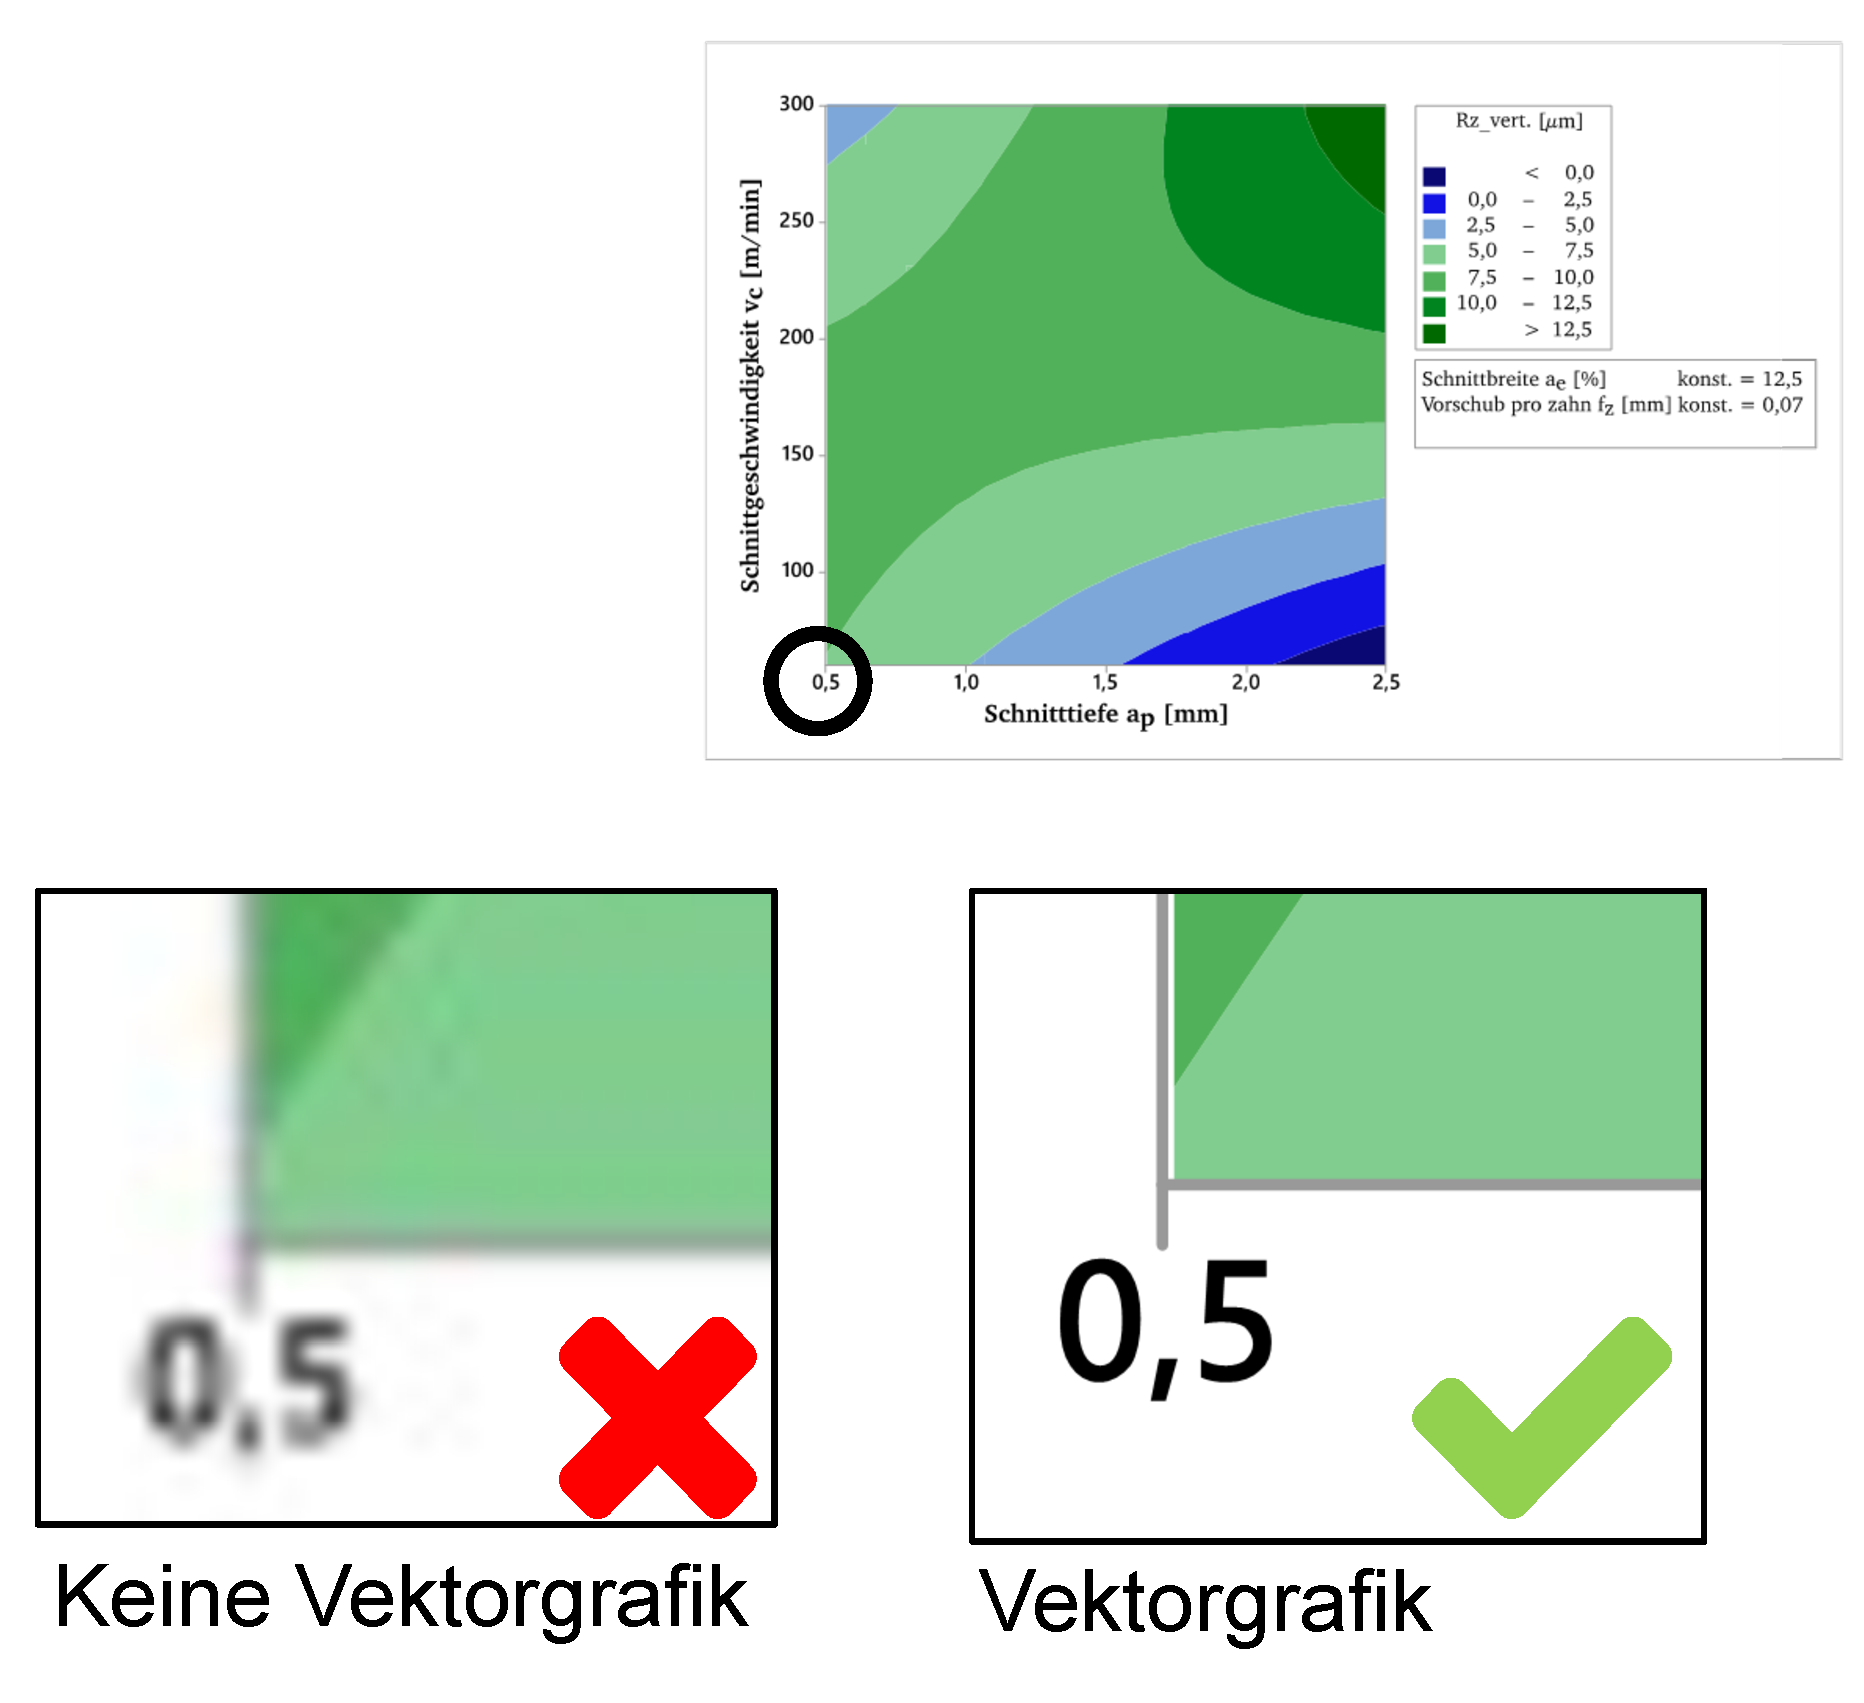
\includegraphics[width=0.5
		\textwidth]{Bilder/Kapt2/Vektorgrafik2.pdf}
		\caption{Vektorgrafik}
		\label{fig:Vektorgrafik}
	\end{center}
\end{figure}

\begin{figure}[H]
	\begin{center}
		\centering
		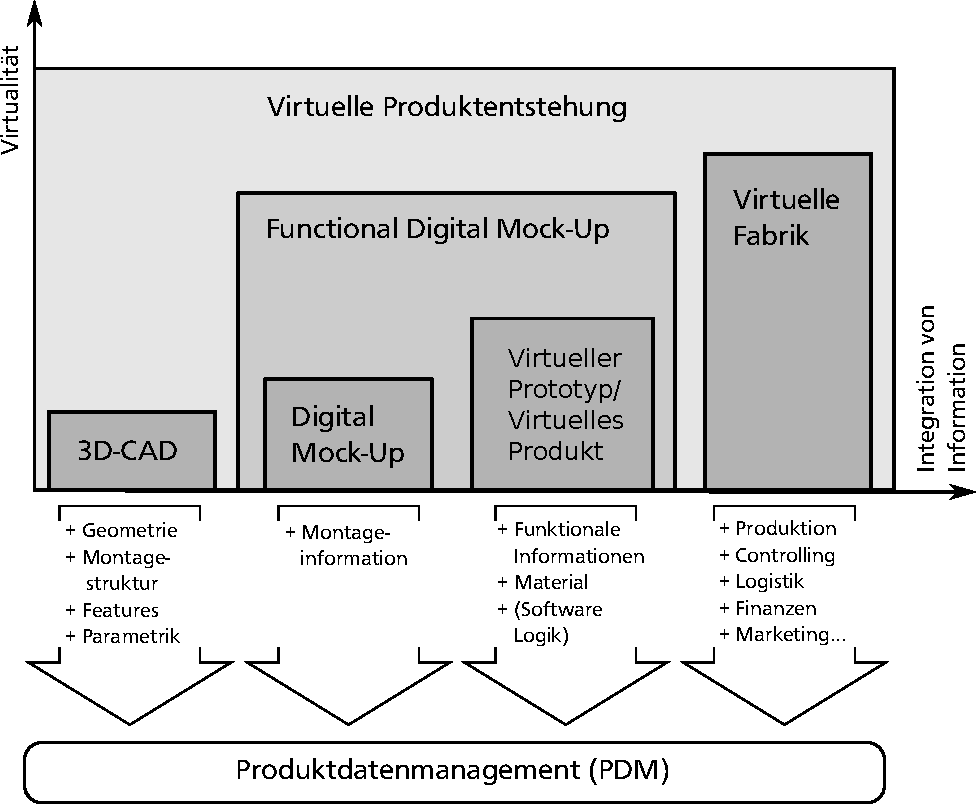
\includegraphics[width=0.6
		\textwidth]{Bilder/Kapt2/EbenenVPEP.pdf}
		\caption{Ebenen der virtuellen Produktentstehung nach \cite{anderl_simulations}}
		\label{fig:EbeneVPEP}
	\end{center}
\end{figure}

\subsection{Tabellen}
Hier der Verweis auf Tab.~\ref{tab:SIM}. Jede Abb. und jede Tab. muss mindestens einmal referenziert werden.
\FloatBarrier
\begin{table}[tbh]
	\centering
	\caption{\centering Simulationen unterschiedlicher Güte}
	\label{tab:SIM}
    \begin{tabular}{l|l|l|l}
	& SIM 1 & SIM 2 & SIM 3 \\
	\hline
	\hline
	Simulationsschritte & 100  & 300 & 3000 \\
	\hline
	Simulationszeit& \SI{50}{s} & \SI{30}{s} & \SI{10}{s} \\
	\hline
	\end{tabular}
\end{table}
\FloatBarrier

\section{Abgabe von Abschlussarbeiten}

\begin{sloppypar}
\begin{itemize}
    \item Die Abgabe der Thesis erfolgt entsprechend der Absprachen mit dem Betreuer einige Wochen vor der finalen und offiziellen Endabgabe.  
    
    \item Der Titel der schriftlichen Ausarbeitung muss identisch mit dem Titel sein, der in TUCaN bei der Anmeldung der Abschlussarbeit steht. 
    
    \item Die offizielle Endabgabe von Abschlussarbeiten erfolgt in elektronischer Form über TUbama (\url{https://tubama.ulb.tu-darmstadt.de/}). Weitere Infos unter: \url{https://www.tu-darmstadt.de/studieren/studierende_tu/studienorganisation_und_tucan/hilfe_und_faq/artikel_details_de_en_96256.de.jsp}
    Hierzu bitte die Vorgaben des MechCenters berücksichtigen.

    \item Weitere Informationen unter TUbama (\url{https://tubama.ulb.tu-darmstadt.de/})

\end{itemize}
\end{sloppypar}


\section{Lernziele von Abschlussarbeiten}

\begin{enumerate}
    \item Eine technisch-wissenschaftliche Fragestellung mit ingenieurwissenschaftlichen Methoden strukturiert zu lösen.
    \item Die Fragestellung kritisch zu bearbeiten und mögliche Lösungen einzuschätzen.
    \item Die Ergebnisse in schriftlicher und mündlicher Form mit wissenschaftlichen Anspruch zu präsentieren.
\end{enumerate}

\subsection*{Grundregeln des wissenschaftlichen Arbeitens}
\begin{itemize}
    \item Ergebnisse, Methoden und Verfahren sorgfältig und nachvollziehbar dokumentieren.
    \item Integre Argumentation bei wissenschaftlichen Auseinandersetzungen
    \begin{itemize}
        \item Klare Unterscheidung von Ergebnissen und deren Interpretation
    \end{itemize}
    \item Verantwortungsvolles Verhalten zwischen Student*in und Betreuer*in
    \item Zitation von Forschungsergebnissen, Publikationen und Ideen anderer Wissenschaftler*innen
    \item Verantwortungsvoller Umgang mit Daten und KI
    \begin{itemize}
        \item Siehe \href{https://www.maschinenbau.tu-darmstadt.de/media/maschinenbau/dokumente_2/studieren_1/thesis/2025-06-20_KI-Leitlinien_FB_MB.de.pdf}{Hilfsmittel} zum Umgang mit KI-Hilfsmitteln des Maschinenbaus.
        \item Siehe \href{https://www.hda.tu-darmstadt.de/hochschuldidaktik/infoseiten_hd/handreichung_ki_hd/handreichung_ki_verteilerseite.de.jsp}{Zentraler KI-Leitfaden} der TU Darmstadt
    \end{itemize}
\end{itemize}
\section{Weitere Links}
\begin{sloppypar}
\begin{itemize}
    \item Schreibgruppen vom SchreibCenter am Sprachenzentrum\\ (\url{https://www.owl.tu-darmstadt.de/angebote_vor_ort/schreibgruppen/schreibgruppen.de.jsp})
    \item Software vom HRZ\\
\url{https://www.hrz.tu-darmstadt.de/services/it_services/campus_software/index.de.jsp}
    \item GitLab Versionsverwaltung\\ \url{https://www.hrz.tu-darmstadt.de/services/it_services/gitlab/index.de.jsp}
    \item Normen und Regelwerke\\
\url{https://www.ulb.tu-darmstadt.de/finden_nutzen/recherchieren/normen_richtlinien.de.jsp}
    \item Kompilierungszeit verringern\\
Um die Kompilierungszeit der einzelnen Dateien zu verringern, kann die Ausarbeitung über das Package \textit{subfiles} organisiert werden. Eine Anleitung für die Umsetzung ist hier zu finden: \url{https://de.overleaf.com/learn/latex/Multi-file_LaTeX_projects}

\end{itemize}
\end{sloppypar}

\section{Modulare Fertigung}
\label{sec:ModulareFertigung}

Produzierende Unternehmen stehen zunehmend vor der Herausforderung, ihre Fertigung an wechselnde Marktanforderungen anzupassen. Eine steigende Produktvielfalt, kürzere Produktlebenszyklen und schwankende Produktionsmengen erfordern Produktionssysteme, die sowohl effizient als auch flexibel betrieben werden können. Klassische, starr aufgebaute Fertigungsanlagen stoßen dabei an ihre Grenzen, da Änderungen häufig mit umfangreichen Umbauten und hohen Kosten verbunden sind. Einen Ansatz zur Bewältigung dieser Herausforderungen bietet die modulare Fertigung \cite{Borgmann2026,Trautner2026}.

Grundlage der modularen Fertigung ist die Aufteilung eines Produktionssystems in einzelne, funktional abgegrenzte Module. Jedes Modul übernimmt dabei eine definierte Aufgabe innerhalb des Gesamtsystems und kann weitgehend unabhängig von anderen Modulen betrieben oder verändert werden. Durch die Kombination unterschiedlicher Module lassen sich verschiedene Anlagenkonfigurationen realisieren. Ziel der Modularisierung ist es, die Abhängigkeiten zwischen einzelnen Systemkomponenten zu reduzieren und dadurch die Anpassungsfähigkeit des Produktionssystems zu erhöhen \cite{Borgmann2026}.

Ein wesentliches Merkmal modularer Systeme ist die Verwendung standardisierter Schnittstellen. Diese ermöglichen den Austausch von Material, Energie und Informationen zwischen den einzelnen Modulen. Durch einheitliche Schnittstellen können Komponenten hinzugefügt, entfernt oder ausgetauscht werden, ohne dass umfangreiche Änderungen am gesamten System erforderlich sind. Gleichzeitig erleichtert die Standardisierung die Integration neuer Komponenten und die Wiederverwendung bereits vorhandener Module \cite{Borgmann2026}.

Borgmann und Henke unterscheiden mehrere Eigenschaften, die zur Wandlungsfähigkeit modularer Produktionssysteme beitragen. Dazu zählen insbesondere die Universalität, Mobilität, Skalierbarkeit, Modularität und Kompatibilität. Universalität beschreibt die Möglichkeit, ein Modul für unterschiedliche Aufgaben einzusetzen. Mobilität bezeichnet dessen Ortsveränderlichkeit, während Skalierbarkeit die Erweiterung oder Reduzierung von Kapazitäten ermöglicht. Die Modularität betrifft den inneren Aufbau der Komponenten, wohingegen die Kompatibilität deren Vernetzungsfähigkeit hinsichtlich Material, Energie und Informationen beschreibt \cite{Borgmann2026}.

Eng mit der Modularität verbunden ist das Konzept der Rekonfigurierbarkeit. Darunter wird die Fähigkeit eines Fertigungssystems verstanden, seine Struktur und Funktionalität an veränderte Anforderungen anzupassen. Dies kann beispielsweise durch den Austausch, die Ergänzung oder die Neuanordnung einzelner Komponenten erfolgen. Rekonfigurierbare Fertigungssysteme (RFS) ermöglichen dadurch eine gezielte Veränderung der verfügbaren Fertigungsfunktionen und Produktionskapazitäten. Neben der mechanischen Anpassung können hierfür auch Änderungen der Steuerungssoftware erforderlich sein \cite{Trautner2026}.

Dabei ist zwischen Flexibilität und Rekonfigurierbarkeit zu unterscheiden. Flexibilität beschreibt die Fähigkeit eines Systems, innerhalb eines bereits vorgesehenen Funktionsumfangs auf unterschiedliche Anforderungen zu reagieren. Rekonfigurierbarkeit ermöglicht hingegen die gezielte Veränderung der Systemstruktur, um zusätzliche oder veränderte Anforderungen zu erfüllen. Ein Beispiel hierfür ist eine Roboterzelle, die durch einen Werkzeugwechsel innerhalb ihres bestehenden Funktionsumfangs für unterschiedliche Bearbeitungsaufgaben umgerüstet werden kann. Wird die Zelle hingegen durch zusätzliche Prozessmodule erweitert und dadurch ihre Systemstruktur verändert, handelt es sich um eine Rekonfiguration \cite{Trautner2026}.

Die Rekonfiguration eines Produktionssystems betrifft jedoch nicht ausschließlich dessen mechanischen Aufbau. Werden Module ausgetauscht oder an anderen Positionen angeordnet, müssen auch die zugehörigen Steuerungs- und Kommunikationsstrukturen angepasst werden \cite{Trautner2026}. Insbesondere bei automatisierten Roboterzellen ist zudem die Kenntnis über Position und Orientierung der eingesetzten Komponenten erforderlich, um deren räumliche Beziehungen korrekt berücksichtigen zu können \cite{Bennulf2025}. Die Verbindung modularer Hardware mit geeigneten Kommunikations- und Lokalisierungstechnologien bildet damit eine wichtige Grundlage für die flexible Rekonfiguration von Roboterzellen.


\section{PLCM: Vision und aktueller Stand}
\label{sec:PLCM Vision}
% DAS Kapitel safe nochmal umbenennen

\section{Modulare Roboterzellen}
\label{sec:Modulare Roboterzellen}
%REVIEW MERIC: Hier fehlt noch eine Einleitung, die erklärt warum wir das erklären

\subsubsection{Mössner FlexCube}

Der Mössner FlexCube (MFC) ist eine modular aufgebaute Roboterbearbeitungszelle der Firma August Mössner GmbH \& Co. KG (siehe Abbildung~\ref{fig:MoessnerFlexCube}). Die Roboterzelle ist für verschiedenste Prozesse, wie beispielsweise Fräsen, Bohren und Schleifen geeignet. Die Zelle besteht aus weitgehend unabhängigen, konfigurierbaren Modulen, die bei veränderten Anforderungen getauscht werden können \cite{MoessnerFlexCube}.

\begin{figure}[htbp]
    \centering
    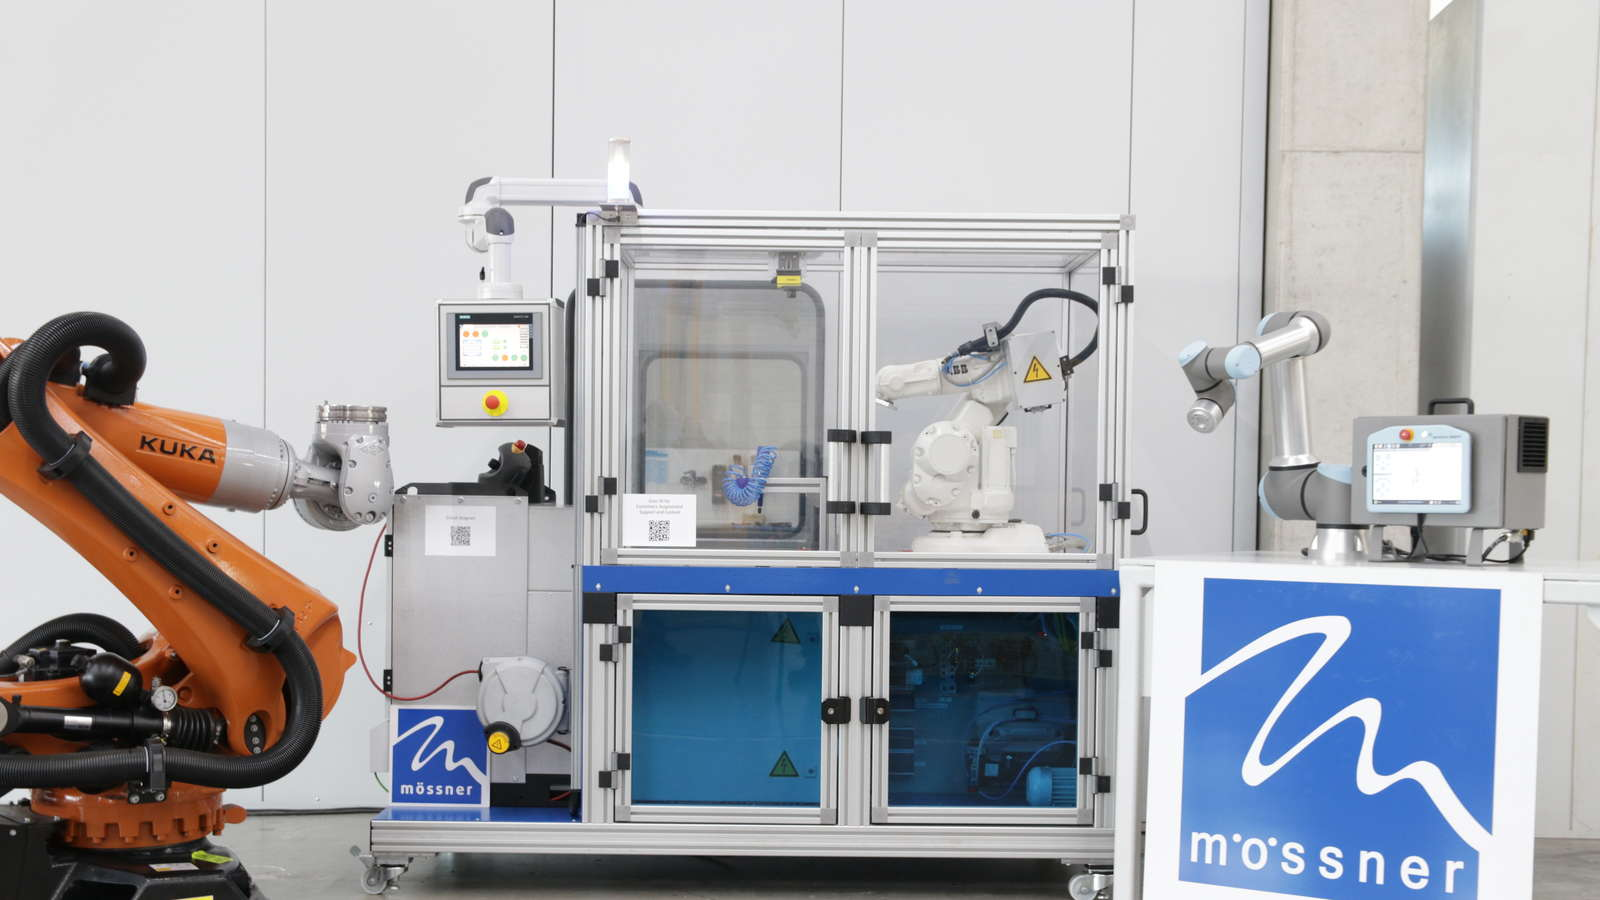
\includegraphics[width=0.75\textwidth]{Bilder/Kapt2/moessner-flex-cube.jpg}
    \caption{Modulare Roboterzelle Mössner FlexCube \cite{MoessnerGIFA2023}}
    \label{fig:MoessnerFlexCube}
\end{figure}

Die Modularität des FlexCube umfasst vor allem, den eingesetzten Roboter, die Werkstückaufnahme, das Werkzeugsystem und die Späneentsorgung. Dabei können Roboter verschiedenster Hersteller wie ABB, FANUC, und KUKA eingesetzt werden. Die Bodenplatte der Roboterzelle ist modular gestaltet und ermöglicht den Austausch der Roboter und Werkstückaufnahmen. Je nach Anwendungsfall stehen unterschiedliche Bearbeitungsspindeln, Werkzeugwechsler sowie Werk- und Drehtische zur Verfügung \cite{MoessnerFlexCube}.

Zusätzlich bietet der Hersteller die Integration kamerabasierter Erkennungssysteme sowie einen digitalen Zwilling zur Simulation und Bewertung von Bearbeitungsprozessen an \cite{MoessnerFlexCube}.

\subsubsection{PoPCoRN}

Im Rahmen des Forschungsprojekts PoPCoRN wird eine rekonfigurierbare Roboterzelle untersucht, bei der Prozessmodule innerhalb weniger Minuten hinzugefügt werden können (siehe Abbildung ~\ref{fig:PoPCoRN}) oder entfernt werden können. Durch standardisierte Anschlüsse und Steuerfunktionen wird eine flexible Anpassung der Zelle an unterschiedliche Fertigungsaufgaben ermöglicht \cite{Bennulf2025}.

\begin{figure}[htbp]
    \centering
    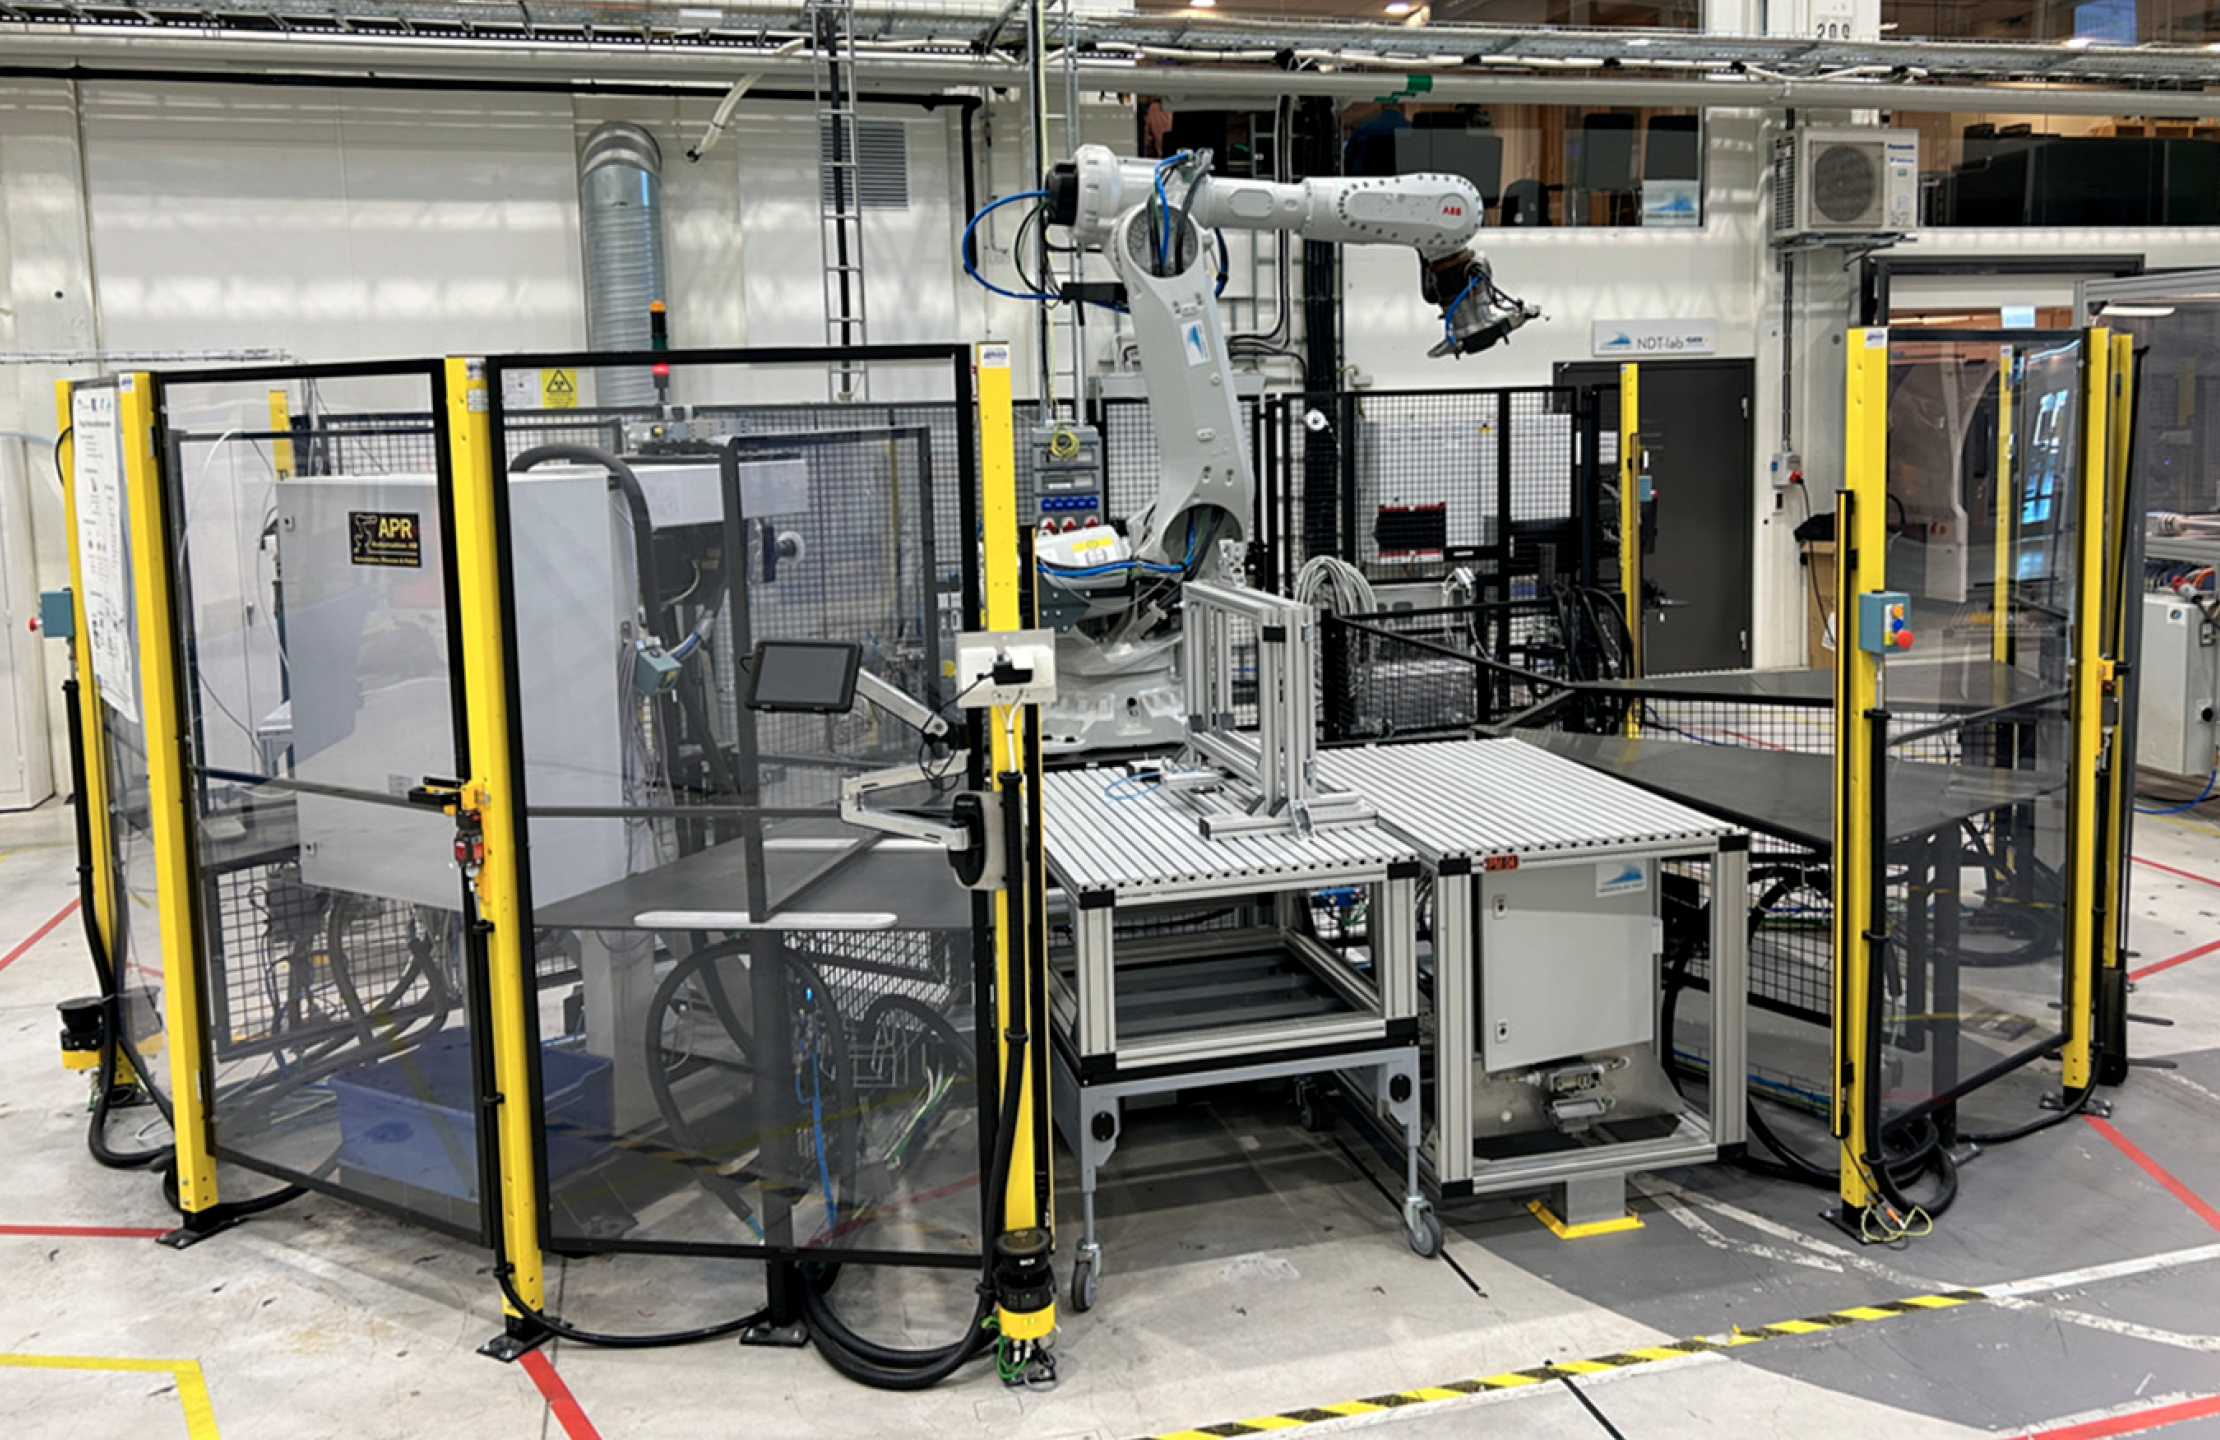
\includegraphics[width=0.75\textwidth]{Bilder/Kapt2/popcorn-aufbau.png}
    \caption{Modulare Plug-and-Produce-Roboterzelle an der University West in Schweden \cite{Bennulf2025}}
    \label{fig:PoPCoRN}
\end{figure}

Bennulf et al. stellen ein Konzept vor, das die automatische Kalibrierung der Modulposition mit der Aktualisierung eines digitalen Zwillings verbindet. Hierzu wird eine am Roboter montierte Kamera verwendet, die ein asymmetrisches Kreismuster auf dem jeweiligen Prozessmodul erfasst. Aus den Bilddaten werden Position und Orientierung des Moduls bestimmt. Die ermittelten Kalibrierungsdaten können anschließend zur Aktualisierung des digitalen Modells und zur automatisierten Bahnplanung verwendet werden \cite{Bennulf2025}.

Die kamerabasierte Kalibrierung wurde an einem physischen Demonstrator experimentell untersucht. Dabei erzielten die Autoren einen maximalen Translationsfehler von etwa 0,43 mm auf einer einzelnen Achse und einen mittleren Fehler von weniger als 0,051 mm \cite{Bennulf2025}.

\section{Kommunikationstechnologien}
\label{sec:Kommunikationstechnologien}

% Wir müssen uns glaube noch bisschen auf einen Stil einigen. Hier sehr professionell, hab es mehr prägnant und einfach geschrieben
Mit der zunehmenden Vernetzung industrieller Produktionssysteme steigt auch der Bedarf an zuverlässigem Informationsaustausch zwischen unterschiedlichen Hardware- und Softwarekomponenten. Besonders in verteilten Systemen, in denen Komponenten verschiedener Hersteller zusammenspielen, stellt die Interoperabilität eine zentrale Herausforderung dar. Standardisierte Kommunikationsprotokolle sind hierbei die Grundlage für die Integration solcher Komponenten und unterstützen damit die Flexibilität, Modularität und Erweiterbarkeit industrieller Anlagen \cite{Gonzalez2019,Profanter2019}.

\subsubsection{Industrial Ethernet}


Unter Industrial Ethernet werden verschiedene Ethernet-basierte Kommunikationsprotokolle zusammengefasst, die in der industriellen Automatisierung eingesetzt werden. Beispiele sind hierbei PROFINET, EtherCAT und EtherNet/IP. Sie dienen der Vernetzung industrieller Komponenten und können, je nach Protokollvariante, auch zeitkritische Kommunikationsanforderungen erfüllen. Ein wesentlicher Vorteil liegt in der breiten Unterstützung der Ethernet-Technologie durch unterschiedliche Hardwareplattformen und Betriebssysteme \cite{Halenar2023,Profanter2019}.

\subsubsection{OPC UA}

Open Platform Communications Unified Architecture (OPC UA) ist ein plattformunabhängiger Kommunikationsstandard, der vor allem in der industriellen Automatisierung Anwendung findet und in der Normenreihe IEC 62541 spezifiziert ist. OPC UA basiert auf einer serviceorientierten Architektur und ermöglicht den herstellerübergreifenden Informationsaustausch zwischen unterschiedlichsten Systemkomponenten \cite{Gonzalez2019}.

% REVIEW Meric: Würde 2 Sätze draus machen: Die Kommunikation kann über eine Client Server architektur erfolgen. Dabie stellt ein Server Informatonen bereit und Clients greifen auf diese zu.
Die Kommunikation kann über eine Client-Server-Architektur erfolgen, das bedeutet, dass ein Server Informationen bereitstellt und Clients auf diese zugreifen. Neben der direkten Datenabfrage können Clients auch Änderungen von Variablen abonnieren. Zusätzlich unterstützt OPC UA das Publish-Subscribe-Modell \cite{Profanter2019,Hlayel2026}.


Eine Besonderheit von OPC UA ist die semantische Beschreibung der bereitgestellten Daten mittels Informationsmodellen. Durch anwendungsspezifische Erweiterungen, die sogenannten Companion Specifications, lassen sich diese Modelle für verschiedene Einsatzbereiche wie die Robotik oder die industrielle Bildverarbeitung standardisieren. Darüber hinaus verfügt OPC UA über integrierte Sicherheitsmechanismen zur Authentifizierung und Verschlüsselung \cite{Gonzalez2019,Profanter2019}.

\subsubsection{MQTT}

Message Queuing Telemetry Transport (MQTT) ist ein nachrichtenbasiertes Protokoll, das insbesondere im Internet of Things (IoT) verbreitet ist. Die Kommunikation folgt dem Publish-Subscribe-Prinzip und wird über eine zentrale Vermittlungsinstanz, den Broker, abgewickelt. Ein Publisher veröffentlicht Nachrichten unter bestimmten Topics, die der Broker an die jeweiligen Subscriber weiterleitet. MQTT zeichnet sich durch einen geringen Ressourcenbedarf und einen sparsamen Bandbreitenverbrauch aus. Verschiedene Quality-of-Service-Stufen (QoS) ermöglichen
zudem eine gezielte Beeinflussung der Zuverlässigkeit der Nachrichtenübertragung \cite{Profanter2019,Hlayel2026}.

\subsubsection{WebSocket}

WebSocket erlaubt einen kontinuierlichen, bidirektionalen Datenaustausch über eine bestehende TCP-Verbindung. Im Gegensatz zur klassischen HTTP-basierten Anfrage-Antwort-Kommunikation können sowohl Client als auch Server selbstständig Nachrichten über die geöffnete Verbindung senden. Diese Kommunikationsform wird als Full-Duplex bezeichnet \cite{Hlayel2026}.

Obwohl WebSocket ursprünglich für die Kommunikation zwischen webbasierten Anwendungen und Servern entwickelt wurde, findet das Protokoll inzwischen auch in der industriellen Automatisierung Anwendung. Hlayel et al. untersuchen beispielsweise eine WebSocket-basierte Schnittstelle zwischen einer speicherprogrammierbaren Steuerung (SPS) und einem digitalen Zwilling. Die persistente Verbindung und der ereignisbasierte Datenaustausch ermöglichen in der untersuchten Architektur eine Kommunikation mit geringer Latenz \cite{Hlayel2026}.

%REVIEW Meric: Eventueller Kreuzverweis auf Relevanz der Technologien zu einem späteren Kapitel, die KI macht das super gerne bei John seiner Masterthesis und ich fande das eigt ganz gut in einem begrenzten Rahmen.
Die betrachteten Technologien unterscheiden sich vor allem in ihrer Kommunikationsarchitektur, ihrem Funktionsumfang und ihren typischen Anwendungsfeldern. Während Industrial Ethernet der netzwerkbasierten Vernetzung industrieller Komponenten dient, unterstützen OPC UA, MQTT und WebSocket den Datenaustausch auf Anwendungsebene \cite{Halenar2023,Profanter2019,Hlayel2026}. Aufgrund ihrer unterschiedlichen Aufgaben können die
Technologien innerhalb eines industriellen Gesamtsystems ergänzend eingesetzt werden.

\section{Lokalisierungstechnologien}
\label{sec:Lokalisierungstechnologien}
\textbf{Vorschlag Einleitung KI:} Für die Lokalisierung von Objekten gibt es verschiedene technische Ansätze, die sich vor allem im Messprinzip unterscheiden. Im Folgenden werden visuelle, ultrabreitbandbasierte und feldbasierte Verfahren vorgestellt. Im Mittelpunkt stehen dabei die erreichbare Genauigkeit, die Größe des abdeckbaren Bereichs und der nötige Installationsaufwand. Abschließend werden die Verfahren gegenübergestellt.
\subsection{Visuelle Lokalisierung}

Visuelle Lokalisierungsverfahren ermöglichen die Bestimmung der Position und Orientierung von Objekten anhand von Bildinformationen. Hierzu werden Kameras eingesetzt, deren Bilddaten mithilfe geeigneter Bildverarbeitungsalgorithmen ausgewertet werden. Eine Möglichkeit zur Lokalisierung besteht in der Verwendung sogenannter Fiducial Marker. Dabei handelt es sich um künstlich erzeugte, visuell eindeutig identifizierbare Markierungen, die an den zu lokalisierenden Objekten angebracht werden. Durch die Erkennung dieser Marker innerhalb eines Kamerabildes können sowohl eine eindeutige Identifikation des jeweiligen Objekts als auch die Bestimmung seiner räumlichen Lage erfolgen \cite{Kalaitzakis2021}.

%REVIEW Meric: Ist das wirklich neutral geschrieben, warum nur Einsatz bei quadratischen Markern. Glaube hier entweder überall, keine oder allgemein. Außerdem dopplung mit dem nächsten Absatz
Fiducial Marker lassen sich hinsichtlich ihrer geometrischen Gestaltung und ihres Erkennungsverfahrens unterscheiden. Zu den grundlegenden Kategorien zählen kreisförmige, quadratische und topologische Marker sowie auf Deep Learning basierende Ansätze. Kreisförmige Marker besitzen aufgrund ihrer Geometrie Eigenschaften, die bei perspektivischen Verzerrungen vorteilhaft sein können. Quadratische Marker sind insbesondere in der Robotik und im Bereich der Augmented Reality weit verbreitet. Topologische Marker ermöglichen die Darstellung einer großen Anzahl unterschiedlicher Identifikationsmuster, während lernbasierte Verfahren trainierte Modelle zur Erkennung und Identifikation der Markierungen einsetzen \cite{Kuzmenko2025}. Abbildung \ref{fig:markerarten} zeigt eine Übersicht der verschiedenen Fiducial-Marker-Typen.

\begin{figure}[H]
    \centering
    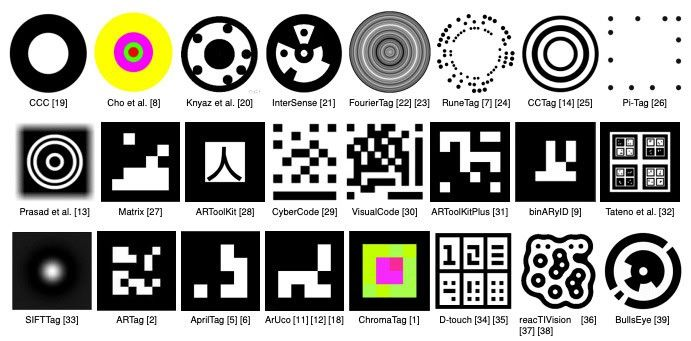
\includegraphics[width=0.9\textwidth]{Bilder/Kapt2/marker-overview.jpg}
    \caption{Übersicht verschiedener Fiducial-Marker-Systeme.
    \cite{Kuzmenko2025}}
    \label{fig:markerarten}
\end{figure}

Für die industrielle Robotik sind insbesondere quadratische Fiducial Marker relevant. Zu den etablierten Verfahren zählen AprilTag, ArUco und ARTag. Diese verwenden charakteristische Muster, anhand derer einzelne Marker identifiziert und ihre Position sowie Orientierung relativ zur Kamera bestimmt werden können. Voraussetzung für eine zuverlässige Positionsbestimmung ist neben der bekannten Markergröße eine geeignete Kalibrierung des Kamerasystems \cite{Kalaitzakis2021}.

%REVIEW Meric: Langer Absatz, eventuell in Ergebnisse und Einflussfaktoren teilen.
% REVIEW Meric: AprilTag schneidet hier schlechter ab als ArUco, wir müssen uns noch eine Brügungun aus dem Arsch ziehen warum wir doch AprilTags genommen haben. @sven @Ming
Die Leistungsfähigkeit verschiedener Fiducial-Marker-Verfahren wurde von Jurado-Rodriguez et al. anhand experimenteller Untersuchungen verglichen. Dabei wurden insgesamt 13 Markererkennungsverfahren hinsichtlich ihrer Positionsgenauigkeit, Erkennungsreichweite, Robustheit gegenüber Verdeckungen und Verarbeitungsgeschwindigkeit untersucht. Die Ergebnisse zeigen, dass insbesondere ArUco3 bei der Positionsbestimmung eine hohe Genauigkeit erreicht. Mit einem mittleren Positionsfehler von \SI{11,5}{\milli\metre} erzielte ArUco3 das beste Ergebnis, gefolgt von STag mit \SI{12,9}{\milli\metre} und ArUco mit \SI{13,2}{\milli\metre}. AprilTag3 und AprilTag2 erreichten dagegen mittlere Positionsfehler von \SI{14,9}{\milli\metre} beziehungsweise \SI{15,9}{\milli\metre}. Diese Werte wurden über die untersuchten Aufnahmen bei unterschiedlichen Aufnahmebedingungen ermittelt, wobei Kamera-Marker-Abstände zwischen \num{1} und \SI{6}{\metre} betrachtet wurden. Die angegebenen mittleren Positionsfehler sind daher nicht als konstante Genauigkeitswerte der jeweiligen Markerverfahren zu verstehen. % REVIEW Meric: Wie sonst?
Auch hinsichtlich der Verarbeitungsgeschwindigkeit zeigte ArUco3 mit 106,1 Bildern pro Sekunde die höchste Leistung. Bei der Untersuchung der zeitlichen Stabilität der erkannten Markerecken erzielten hingegen AprilTag3 und AprilTag2 die besten Ergebnisse. Die erzielbare Positionsgenauigkeit hängt darüber hinaus wesentlich von den jeweiligen Versuchsbedingungen ab. Insbesondere der Abstand zwischen Kamera und Marker, die Markerkantenlänge, die Kameraauflösung sowie der Betrachtungswinkel beeinflussen die Genauigkeit der Positionsbestimmung. %REVIEW Meric: Hab das Gefühl, wenn wir das hier so benennen müssen wir das bei uns ein wenig mehr prüfen für Kapital 5
Abbildung \ref{fig:markeraccuracy} zeigt den Einfluss des Kamera-Marker-Abstands und des Betrachtungswinkels auf den Positionsfehler der untersuchten Markerverfahren. Dabei ist zu erkennen, dass der Positionsfehler mit zunehmendem Abstand sowie bei abnehmendem Betrachtungswinkel tendenziell ansteigt. Insbesondere ArUco3 weist über einen großen Teil der untersuchten Abstände und Betrachtungswinkel vergleichsweise geringe Positionsfehler auf \cite{JuradoRodriguez2023}. %REVIEW Meric: Warum ist ArUco hier eigt die ganze das beste, wir müssen das uns irgendwie zurecht legen, warum wir AprilTags genutzt haben. Andere Quellen oder so haha

\begin{figure}[H]
    \centering
    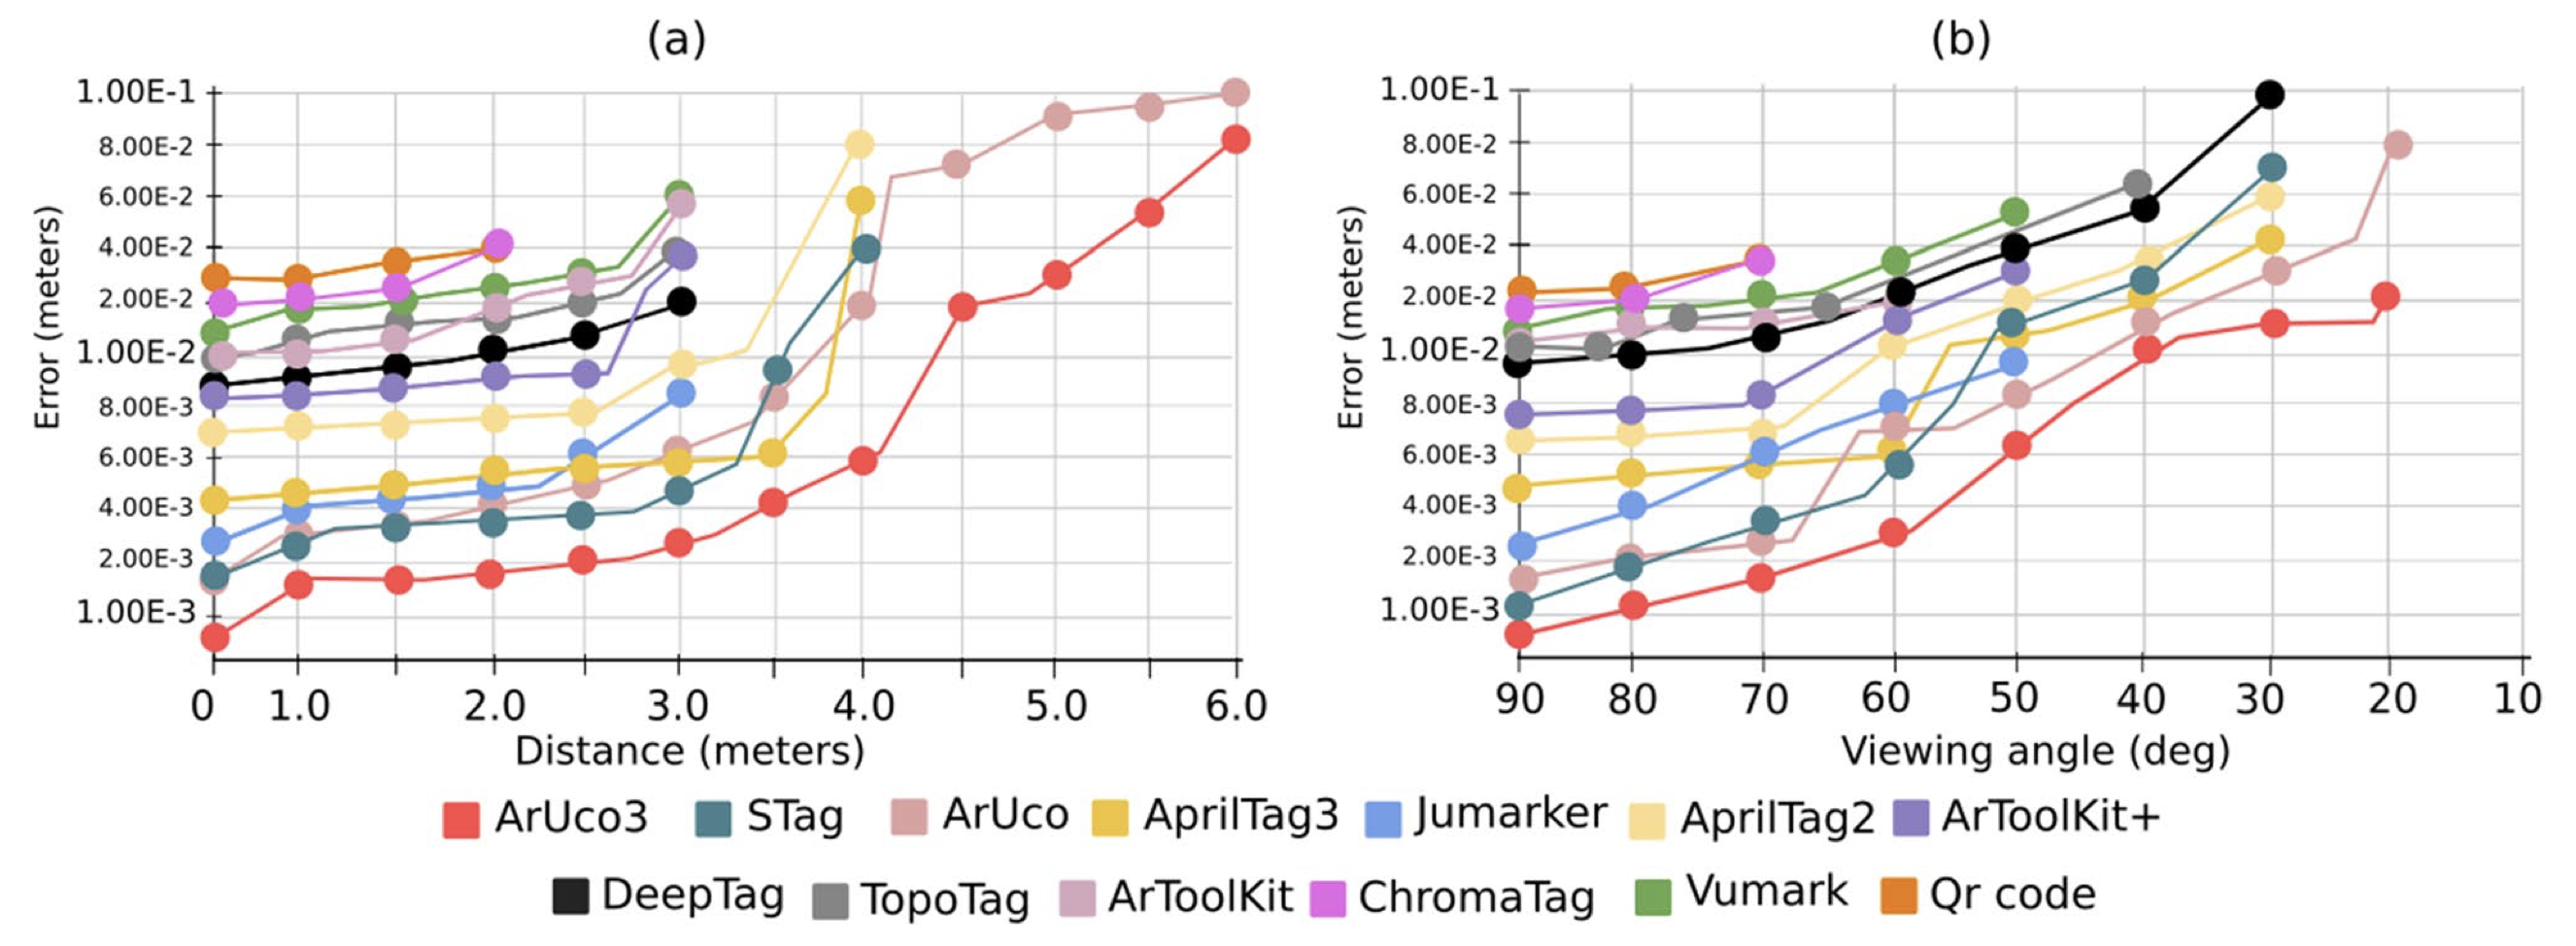
\includegraphics[width=\textwidth]{Bilder/Kapt2/marker-distance.png}
    \caption{Einfluss (a) des Kamera-Marker-Abstands
    und (b) des Betrachtungswinkels auf den
    Positionsfehler verschiedener Fiducial-Marker-Verfahren.
    \cite{JuradoRodriguez2023}}
    \label{fig:markeraccuracy}
\end{figure}
%REVIEW Meric: Auch das scheiß Diagramm sagt, dass wir rmit ArUco3 besser währen, laut dem Diagramm kommen wir mit AprilTags net mal auf unsere geforderte Auflösung. Hab langsam das gefühl wir müssen neue Tags drucken und den Code minimal umbauen vielleicht klappt es dann am Ende

% REVIEW Meric: "erscheint daher grundsätzlich möglich" ist vage. Würde sowas wie daraus sieht man, dass Verbesserung der Lokalisierung bis zu unter einem mm ge anu sind.
% REVIEW John: ich denke man sollte auf jeden Fall wie der AprilTag bei diesen Versuchen aussah, also was die Kantenlaenge war, da es ein Essenzieller Parameter auch bei unserer Untersuchung war.
Die Untersuchung verdeutlicht somit, dass die Eignung eines Markererkennungsverfahrens sowohl von dessen Genauigkeit, Stabilität und Verarbeitungsgeschwindigkeit als auch von den konkreten Einsatzbedingungen abhängt. Insbesondere Abbildung \ref{fig:markeraccuracy} zeigt, dass bei geringen Kamera-Marker-Abständen deutlich niedrigere Positionsfehler erzielt werden als bei größeren Entfernungen. So lässt sich für ArUco3 bei einem Abstand von \SI{1}{\metre} ein Positionsfehler von etwa \SI{1,7}{\milli\metre} ablesen, während der über die verschiedenen Versuchsbedingungen gemittelte Positionsfehler \SI{11,5}{\milli\metre} beträgt. Für Anwendungen mit Abständen unter \SI{1}{\metre} erscheint daher eine weitere Verbesserung der Genauigkeit grundsätzlich möglich.

\subsection{Ultrabreitbandbasierte Lokalisierung}

%REVIEW Meric: HAb die Einheiten zu SI Einheiten gemacht, würde vergleichweise streichen
Ultra-Wideband (UWB) ist eine funkbasierte Technologie, die zur drahtlosen Kommunikation und zur Positionsbestimmung von Objekten eingesetzt werden kann. Im Gegensatz zu schmalbandigen Funktechnologie nutzt UWB Signale mit einer besonders großen Bandbreite von mindestens \SI{500}{\mega\hertz} beziehungsweise einer relativen Bandbreite von mindestens \SI{20}{\percent}. Insbesondere bei impulsbasierten UWB-Verfahren ermöglichen kurze Funkimpulse eine hohe zeitliche Auflösung der Signallaufzeitmessung und damit eine vergleichsweise präzise Abstandsmessung \cite{Elsanhoury2022}.


Die Positionsbestimmung erfolgt typischerweise mithilfe mehrerer Referenzstationen, sogenannter Anchors, deren räumliche Positionen bekannt sind. Das zu lokalisierende Objekt wird mit einem UWB-Sender beziehungsweise Tag ausgestattet, der Funksignale mit den Referenzstationen austauscht. Aus den empfangenen Signalen können mithilfe unterschiedlicher Verfahren Informationen über die Entfernung zu den einzelnen Referenzstationen gewonnen werden. Zu den verbreiteten Methoden zählen Time of Arrival (ToA), Time Difference of Arrival (TDoA) und Two-Way Ranging (TWR). Während ToA auf der Messung der absoluten Signallaufzeit basiert, werden bei TDoA die Laufzeitunterschiede zwischen mehreren Empfangsstationen ausgewertet. TWR ermöglicht dagegen die Entfernungsschätzung anhand eines Signalaustauschs zwischen zwei Geräten \cite{Elsanhoury2022}.

Bei der laufzeitbasierten Entfernungsmessung ergibt sich der Abstand zwischen Sender und Empfänger grundsätzlich aus der Ausbreitungsgeschwindigkeit des Funksignals und dessen Laufzeit:

\begin{equation}
    d = c \cdot \Delta t
    \label{eq:uwb_distance}
\end{equation}

%REVIEW Meric: Da Adrian meinte wir sollen uns kurz fassen beim Stand der Technik sehe ich hier bisschen einsparpotential. Einfach alles bisschen komprimieren. Trilateration in 2-3 knappen Sätzen
Dabei bezeichnet \(d\) die Entfernung zwischen Sender und Empfänger, \(c\) die Lichtgeschwindigkeit und \(\Delta t\) die einfache Signallaufzeit. Bei Two-Way Ranging (TWR) wird diese unter Berücksichtigung der Antwortverzögerung aus der gemessenen Hin- und Rücklaufzeit ermittelt. Durch die Kombination mehrerer Entfernungsmessungen zu bekannten Referenzstationen kann anschließend mithilfe der Trilateration die Position des Objekts bestimmt werden. Für die dreidimensionale Positionsbestimmung werden typischerweise mindestens vier geeignet angeordnete Referenzstationen eingesetzt. Bei bekannten Entfernungen können unter geeigneten geometrischen Bedingungen auch drei Referenzstationen ausreichen, sofern die Mehrdeutigkeit der Positionslösung aufgelöst werden kann. Muss zusätzlich eine unbekannte Zeitabweichung geschätzt werden, sind weitere unabhängige Messungen erforderlich. Die Genauigkeit der Positionsschätzung hängt dabei unter anderem von der räumlichen Anordnung der Referenzstationen und der Genauigkeit der einzelnen Entfernungsmessungen ab
\cite{Elsanhoury2022}.


%REVIEW Meric: IST AoA und RSS relevant insbesondere RSS klingt sehr ungenau, weil ich schätze es fällt mit r^3 ab. Hier eventuell prägantner
Ein wesentlicher Vorteil der UWB-Technologie liegt in ihrer vergleichsweise hohen Genauigkeit gegenüber vielen anderen funkbasierten Lokalisierungsverfahren. Elsanhoury et al. beschreiben für Anwendungen in der Indoor-Logistik Positionsgenauigkeiten im Bereich von etwa \SIrange{5}{30}{\centi\metre}. Die tatsächlich erreichbare Genauigkeit ist jedoch von der eingesetzten Hardware, dem Lokalisierungsverfahren und den Umgebungsbedingungen abhängig. Insbesondere in industriellen Umgebungen können metallische Objekte und andere Hindernisse durch Signalreflexionen und Abschattungen die Positionsbestimmung beeinträchtigen. Neben den laufzeitbasierten Verfahren kann die Positionsbestimmung auch anhand der Einfallswinkel empfangener Funksignale (Angle of Arrival, AoA) oder der empfangenen Signalstärke (Received Signal Strength, RSS) erfolgen. Während bei AoA die Einfallsrichtung des Signals bestimmt wird, dient bei RSS die empfangene Signalstärke zur Abschätzung der Entfernung zwischen Sender und Empfänger \cite{Elsanhoury2022}. Abbildung \ref{fig:uwb_localization} veranschaulicht die unterschiedlichen Verfahren der funkbasierten Positionsbestimmung anhand von Einfallswinkeln, Entfernungen und Signallaufzeitdifferenzen.

\begin{figure}[H]
    \centering
    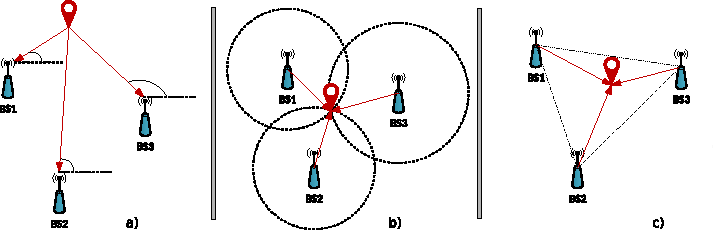
\includegraphics[width=\textwidth]{Bilder/Kapt2/UWB.pdf}
    \caption{Verfahren zur funkbasierten Positionsbestimmung:
    (a) Angle of Arrival (AoA),
    (b) Time of Arrival (ToA), Two-Way Ranging (TWR)
    und Received Signal Strength (RSS) sowie
    (c) Time Difference of Arrival (TDoA).
    \cite{Elsanhoury2022}}
    \label{fig:uwb_localization}
\end{figure}

Eine besondere Herausforderung stellen sogenannte Non-Line-of-Sight-Bedingungen (NLOS) dar, bei denen keine direkte Sichtverbindung zwischen Sender und Empfänger besteht. In solchen Situationen können Funksignale über reflektierte Ausbreitungswege empfangen werden, wodurch sich die gemessene Signallaufzeit gegenüber dem direkten Übertragungsweg erhöht. Dies kann zu systematischen Fehlern bei der Entfernungsschätzung und damit zu einer ungenauen Positionsbestimmung führen. Trotz der vergleichsweise guten Eigenschaften von UWB bei Mehrwegausbreitung können solche Fehler nicht vollständig vermieden werden \cite{Elsanhoury2022}.

UWB-basierte Lokalisierungssysteme werden insbesondere zur Positionsbestimmung von Fahrzeugen, mobilen Robotern, Materialien und anderen Ressourcen in industriellen Innenräumen eingesetzt. Die Technologie ermöglicht eine funkbasierte Ortung ohne kamerabasierte Erkennung und ist daher nicht unmittelbar von den Beleuchtungsverhältnissen abhängig. 
%REVIEW Meric: Trivial dass es keine Kamera hat würde ich nicht schreiben.
Allerdings erfordert die Positionsbestimmung die Installation geeigneter Referenzstationen sowie die Ausstattung der zu lokalisierenden Objekte mit entsprechender Hardware \cite{Elsanhoury2022}.

Bei konventionellen laufzeitbasierten UWB-Systemen wird zunächst die räumliche Position eines einzelnen Tags bestimmt. Aus dieser Position allein lässt sich die vollständige Orientierung eines Moduls jedoch nicht ableiten. Hierfür sind zusätzliche Informationen erforderlich. Chen et al. zeigen, dass durch den Einsatz mehrerer räumlich getrennter UWB-Tags mit bekannter geometrischer Anordnung sowohl die Position als auch die Orientierung eines Objekts bestimmt werden können \cite{Chen2025UWB}.

Zusammenfassend stellt UWB eine Möglichkeit zur flexiblen Positionsbestimmung von Objekten innerhalb industrieller Umgebungen dar. Während die Technologie insbesondere bei der Lokalisierung beweglicher Ressourcen und größerer Arbeitsbereiche Vorteile bietet, müssen bei Anwendungen mit hohen Anforderungen an die Positions- und Orientierungsgenauigkeit die erreichbare Messgenauigkeit, die erforderliche Infrastruktur sowie mögliche Störeinflüsse berücksichtigt werden.

\subsection{Feldbasierte Lokalisierung}

\textbf{Vorschlag KI:} Feldbasierte Verfahren bestimmen die Lage eines Objekts über ein elektromagnetisches oder magnetisches Feld. Gemessen wird dabei nur in einem begrenzten Nahbereich um das Lesegerät oder den Sensor. Im Folgenden werden mit dem RFID-Grid und dem Hall-Sensor-Array zwei Vertreter dieses Prinzips vorgestellt.



\subsubsection{RFID-Grid}

Radio Frequency Identification (RFID) ist eine funkbasierte Technologie, mit der sich Objekte kontaktlos über elektromagnetische Felder identifizieren lassen. Ein typisches System besteht aus einem Lesegerät (Reader) mit Antenne und einem Transponder, dem RFID-Tag. Jeder der verwendeten RFID-Tags besitzt eine eindeutige Kennung, die das Lesegerät erfasst und einem bestimmten Objekt oder einer bekannten Position zuordnen kann. Bei passiven Tags erfolgt die Energieversorgung ausschließlich über das Feld des Readers, sodass keine eigene Stromquelle nötig ist \cite{MiTakahashi2016}.

Für die Positionsbestimmung können die Tags in einem regelmäßigen räumlichen Raster angeordnet werden, dem sogenannten RFID-Grid. Die Positionen der einzelnen Tags sind dabei bekannt und werden in einer Karte hinterlegt. Ein mit RFID-Lesegeräten ausgestatteter Roboter liest die Kennungen der Tags in seinem Erfassungsbereich und kann daraus Informationen über seine eigene Position ableiten. Mi und Takahashi beschreiben ein solches System, bei dem passive Tags rasterförmig im Boden installiert und mehrere Reader an der Unterseite eines mobilen Roboters angebracht sind \cite{MiTakahashi2016}. Abbildung~\ref{fig:rfid_grid} veranschaulicht die Anordnung der RFID-Tags und des mobilen Roboters.

\begin{figure}[H]
    \centering
    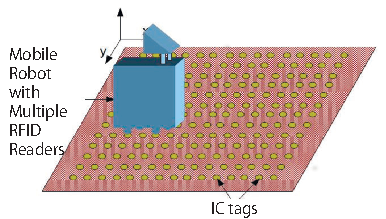
\includegraphics[width=0.65\textwidth]{Bilder/Kapt2/RFID-Grid.pdf}
    \caption{Prinzip der RFID-Grid-basierten
    Lokalisierung eines mobilen Roboters
    anhand rasterförmig angeordneter
    RFID-Tags \cite{MiTakahashi2016}.}
    \label{fig:rfid_grid}
\end{figure}

%REVIEW Meric: der MCL Teil scheint mir sehr bezogen auf Roboter zu sein und nicht direkt auf unser Problem, da wir recht stationär sind.
Die eigentliche Lokalisierung erfolgt über die Zuordnung der erkannten Tag-IDs zu den bekannten Koordinaten im Raster. Da die bloße Erkennung eines Tags nur anzeigt, dass sich dieser im Erfassungsbereich eines Readers befindet, lässt sich die exakte Position nicht aus einer einzelnen Messung ableiten. Für eine genauere Schätzung werden daher mehrere Messungen und Informationen über die Bewegung des Roboters einbezogen. Mi und Takahashi setzen hierzu die Monte-Carlo-Lokalisierung (MCL) ein, ein probabilistisches Verfahren, das mögliche Positionen und Orientierungen anhand eines Bewegungsmodells und der beobachteten Tags bewertet. Auf diese Weise können sowohl die Position als auch die Orientierung des Roboters in der Ebene geschätzt werden \cite{MiTakahashi2016}.

%REVIEW Meric: Glaube das mobile Roboterpaper ist kacke für unseren Use Case, aber alles umschreiben will ich auch net xD
Die erreichbare Genauigkeit hängt unter anderem von der Dichte und Anordnung der Tags, der Zahl und Größe der Reader-Antennen sowie dem gewählten Lokalisierungsverfahren ab. In den Untersuchungen von Mi und Takahashi kam ein HF-RFID-System mit acht Lesegeräten und passiven Tags zum Einsatz, die mit 100 bzw. 16 Tags pro Quadratmeter im Boden verteilt waren. Zur experimentellen Bestimmung der Lokalisierungsfehler
wurde die Position des Roboters an acht bekannten Messpunkten ausgewertet, wobei der Roboter an jedem Messpunkt für \SI{20}{\second} angehalten wurde. Bei der höheren Dichte von 100 Tags/m² ergaben sich mit dem kombinierten Wahrscheinlichkeitsmodell mittlere Fehler von \SI{4,7}{\milli\metre} in x-Richtung und \SI{22,8}{\milli\metre} in y-Richtung. Bei der geringeren Dichte von 16 Tags/m² lagen die mittleren Abweichungen bei \SI{13,0}{\milli\metre} bzw. \SI{8,7}{\milli\metre}. Die Ergebnisse verdeutlichen, dass auch bei einer geringeren Tag-Dichte unter den untersuchten Bedingungen eine Lokalisierung mit vergleichsweise geringen Abweichungen möglich ist. Allerdings treten bei niedrigerer Dichte teilweise größere maximale Abweichungen auf \cite{MiTakahashi2016}.

%REVIEW Meric: Wieder trivial mit Licht würde ich so nicht nennen.
Ein klarer Vorteil der RFID-Grid-Lokalisierung liegt darin, dass die Identifikation der Tags ohne optische Sensoren auskommt und damit weitgehend unabhängig von den Lichtverhältnissen ist. Passive Tags ermöglichen zudem die Installation zahlreicher Referenzpunkte, ohne dass an jedem einzelnen eine Energieversorgung vorgesehen werden muss. Demgegenüber steht der Aufwand für die Installation des Rasters und die Notwendigkeit, die genauen Positionen aller Tags zu kennen. Außerdem beeinflussen die Erfassungsbereiche der Reader und mögliche Störungen bei der Tag-Erkennung sowohl die Genauigkeit als auch die Zuverlässigkeit der Positionsbestimmung \cite{MiTakahashi2016}.

%REVIEW Meric: Fazit gefällt mir sehr, hatte viele Kommentare geschrieben, dass wir uns mit dem mobilen Roboter bisschen f**ken. Aber würde genau deswegen oben die Abschnitte stark kürzen, weil es halt alles auf einen mobilen Roboter sich bezieht und wir daraum nur die grundlegende Idee dahinter erklären sollten.
RFID-Grid-Systeme eignen sich damit grundsätzlich zur Lokalisierung von Objekten in strukturierten Umgebungen. Die untersuchten Ansätze sind vor allem für mobile Roboter gedacht, die sich über einem bekannten Tag-Raster bewegen. Für die Lokalisierung modularer Komponenten innerhalb einer Roboterzelle wäre eine entsprechende Anpassung der Tag- und Reader-Anordnung erforderlich. Dabei ist zu beachten, dass die in der Literatur berichteten Genauigkeiten stark von der jeweiligen Systemkonfiguration abhängen und nicht ohne Weiteres auf andere Anwendungen übertragbar sind.

\subsubsection{Hall-Sensor-Array}

Hall-Sensoren ermöglichen die kontaktlose Erfassung magnetischer Felder und können zur Positionsbestimmung von Objekten eingesetzt werden. Sie basieren auf dem Hall-Effekt und liefern ein elektrisches Ausgangssignal in Abhängigkeit von der magnetischen Flussdichte. Werden mehrere Hall-Sensoren in einer definierten räumlichen Anordnung kombiniert, entsteht ein sogenanntes Hall-Sensor-Array. Durch die Auswertung der Messsignale mehrerer Sensoren können Informationen über die Position einer magnetischen Quelle gewonnen werden. Hall-Sensoren zeichnen sich unter anderem durch ihre kompakte Bauform und vergleichsweise geringen Kosten aus \cite{KawatoKim2005}.

Ein mögliches Lokalisierungsprinzip besteht darin, das zu lokalisierende Objekt mit einem Permanentmagneten auszustatten und dessen Magnetfeld mithilfe eines stationären Sensorarrays zu erfassen. Die einzelnen Sensoren messen die magnetische Flussdichte an unterschiedlichen räumlichen Positionen. Da sich die gemessenen Feldstärken mit der Position und Orientierung des Magneten verändern, kann aus der Kombination der Messwerte auf dessen räumliche Lage geschlossen werden. Song et al. untersuchen ein solches System, bei dem ein Permanentmagnet an der Spitze eines flexiblen Roboters angebracht ist. Ein darunter angeordnetes magnetisches Sensorarray erfasst das Magnetfeld und ermöglicht so die Positionsbestimmung der Roboterspitze \cite{Song2026Magnetic}. Abbildung~\ref{fig:hall_localization} zeigt den prinzipiellen Aufbau einer magnetfeldbasierten Lokalisierung mit einem Permanentmagneten und einem stationären Sensorarray.

\begin{figure}[H]
    \centering
    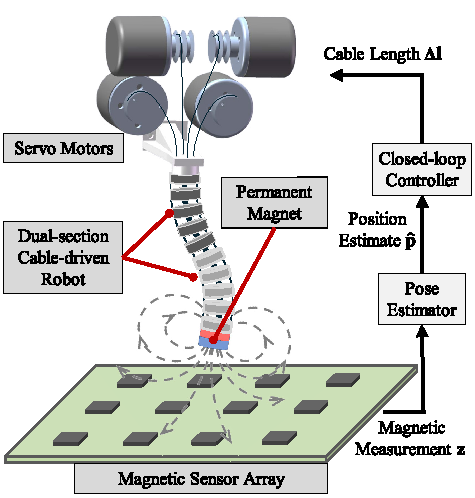
\includegraphics[width=0.6\textwidth]{Bilder/Kapt2/Hall-Array.pdf}
    \caption{Magnetfeldbasierte Lokalisierung
    eines flexiblen Roboters mit Permanentmagnet
    und stationärem Sensorarray
    (aus \cite{Song2026Magnetic}, Abb.~1).}
    \label{fig:hall_localization}
\end{figure}

Für die eigentliche Positionsberechnung können unterschiedliche Auswerteverfahren eingesetzt werden. Song et al. verwenden ein mathematisches Magnetfeldmodell und einen erweiterten Kalman-Filter (Extended Kalman Filter, EKF), um aus den Sensormessungen die dreidimensionale Position des Permanentmagneten zu schätzen \cite{Song2026Magnetic}. Einen anderen Ansatz verfolgen Németh et al., die ein Hall-Sensor-Array mit einem neuronalen Netz kombinieren. Dabei werden die Messwerte mehrerer Hall-Sensoren als Eingangsgrößen eines zuvor trainierten Regressionsmodells verwendet, das daraus die Position des Magneten vorhersagt. Das Modell wird auf einem Mikrocontroller ausgeführt und ermöglicht somit die Positionsschätzung ohne einen externen Hochleistungsrechner \cite{Nemeth2025Hall}.

Neben der Position kann unter geeigneten Bedingungen auch die Orientierung eines Körpers aus magnetischen Messungen bestimmt werden. Kawato und Kim untersuchen hierzu einen magnetisch gelagerten Positioniertisch, der sich über einer Halbach-Magnetmatrix bewegt. Zwei zweiachsige Hall-Sensoren erfassen dabei unterschiedliche Komponenten des räumlich veränderlichen Magnetfeldes. Mithilfe eines modellbasierten Auswerteverfahrens, der Gaussian Least Squares Differential Correction (GLSDC), bestimmen die Autoren sowohl die Position in der Ebene als auch den Rotationswinkel um die vertikale Achse. Die Untersuchung zeigt damit die Möglichkeit einer magnetfeldbasierten Positions- und Orientierungsbestimmung in drei Freiheitsgraden \cite{KawatoKim2005}.

Die erreichbare Genauigkeit hängt von der jeweiligen Systemkonfiguration und dem eingesetzten Auswerteverfahren ab. Kawato und Kim berichten für ihren magnetisch gelagerten Positioniertisch nach entsprechender Kalibrierung eine Positionsauflösung im Bereich unter \SI{10}{\micro\metre} sowie einen maximalen Positionsfehler von etwa \SI{1,4}{\milli\metre} \cite{KawatoKim2005}. Song et al. erreichen bei der Lokalisierung der Spitze eines flexiblen Roboters einen Positionsfehler von ungefähr \SI{3}{\milli\metre}. Die mithilfe dieser Positionsinformationen realisierte geschlossene Regelung weist bei den untersuchten Bewegungsbahnen einen Positionsregelungsfehler von etwa \SI{5}{\milli\metre} auf \cite{Song2026Magnetic}.
%REVIEW Meric: Der Positionsregelfehler scheint mir nicht so relevant zu sein, würde den Satz streichen.
Németh et al. berichten für die Positionsvorhersage ihres neuronalen Netzes mittlere absolute Fehler zwischen \num{0,0263} und \SI{0,0381}{\milli\metre} innerhalb der untersuchten Versuchskonfiguration. Diese Ergebnisse beziehen sich auf ein magnetisches Schwebesystem mit einem begrenzten Arbeitsbereich und lassen sich daher nicht unmittelbar auf andere Anwendungen übertragen \cite{Nemeth2025Hall}.

%REVIEW Meric: Trivial, warum hatest du die optische Sichtverbindung so
Ein Vorteil der magnetfeldbasierten Lokalisierung besteht darin, dass keine optische Sichtverbindung zwischen Sensoren und dem zu lokalisierenden Objekt erforderlich ist. Bei Verwendung eines Permanentmagneten benötigt das Objekt zudem weder eine eigene Energieversorgung noch eine elektrische Verbindung zur Sensorik. Allerdings ist die erreichbare Lokalisierungsgenauigkeit unter anderem vom Abstand zwischen Magnet und Sensorarray sowie von der räumlichen Anordnung der Sensoren abhängig. Song et al. weisen außerdem darauf hin, dass externe magnetische Störfelder, beispielsweise durch ferromagnetische Objekte oder elektronische Geräte, die Positionsschätzung beeinträchtigen können \cite{Song2026Magnetic}. 
%REVIEW Meric: Würde Temperatur noch hinzufügen, aber Sensorausgangsfehler und Rauschen sind glaube allgemeine Fehler die nicht extra genannt werden müssen.
Auch Sensorausgangsfehler, Rauschen und Temperatureinflüsse können die Messgenauigkeit begrenzen \cite{KawatoKim2005}.

%REVIEW Meric: Fazit finde ich top
Hall-Sensor-Arrays stellen somit eine Möglichkeit zur kontaktlosen Lokalisierung magnetisch markierter Objekte dar. Die untersuchten Verfahren zeigen, dass sowohl die Positionsbestimmung als auch unter geeigneten Bedingungen die Erfassung der Orientierung möglich ist. Bei einer Übertragung auf die Lokalisierung modularer Komponenten innerhalb einer Roboterzelle wären insbesondere die Anordnung der Sensoren, die Positionierung der Magnete sowie mögliche magnetische Störeinflüsse zu berücksichtigen. Die in den Untersuchungen erzielten Genauigkeiten sind dabei an die jeweiligen experimentellen Bedingungen gebunden und können nicht ohne Weiteres auf eine andere Systemkonfiguration übertragen werden.

\subsection{Gegenüberstellung der Lokalisierungstechnologien}
%REVIEW Meric: Was ist hier geplant eine Tabelle oder so was? Die wir dann im nächsten Kapitel aufgreifen? Würde es definitiv kompakt machen. MIt Tabelle 1 Seite maximal

